
%% bare_jrnl.tex
%% V1.4b
%% 2015/08/26
%% by Michael Shell
%% see http://www.michaelshell.org/
%% for current contact information.
%%
%% This is a skeleton file demonstrating the use of IEEEtran.cls
%% (requires IEEEtran.cls version 1.8b or later) with an IEEE
%% journal paper.
%%
%% Support sites:
%% http://www.michaelshell.org/tex/ieeetran/
%% http://www.ctan.org/pkg/ieeetran
%% and
%% http://www.ieee.org/

%%*************************************************************************
%% Legal Notice:
%% This code is offered as-is without any warranty either expressed or
%% implied; without even the implied warranty of MERCHANTABILITY or
%% FITNESS FOR A PARTICULAR PURPOSE! 
%% User assumes all risk.
%% In no event shall the IEEE or any contributor to this code be liable for
%% any damages or losses, including, but not limited to, incidental,
%% consequential, or any other damages, resulting from the use or misuse
%% of any information contained here.
%%
%% All comments are the opinions of their respective authors and are not
%% necessarily endorsed by the IEEE.
%%
%% This work is distributed under the LaTeX Project Public License (LPPL)
%% ( http://www.latex-project.org/ ) version 1.3, and may be freely used,
%% distributed and modified. A copy of the LPPL, version 1.3, is included
%% in the base LaTeX documentation of all distributions of LaTeX released
%% 2003/12/01 or later.
%% Retain all contribution notices and credits.
%% ** Modified files should be clearly indicated as such, including  **
%% ** renaming them and changing author support contact information. **
%%*************************************************************************


% *** Authors should verify (and, if needed, correct) their LaTeX system  ***
% *** with the testflow diagnostic prior to trusting their LaTeX platform ***
% *** with production work. The IEEE's font choices and paper sizes can   ***
% *** trigger bugs that do not appear when using other class files.       ***                          ***
% The testflow support page is at:
% http://www.michaelshell.org/tex/testflow/


\documentclass[journal]{IEEEtran}
%
% If IEEEtran.cls has not been installed into the LaTeX system files,
% manually specify the path to it like:
% \documentclass[journal]{../sty/IEEEtran}
\usepackage{color}
\usepackage{graphicx}
\usepackage{subfigure}
\usepackage{threeparttable}
\usepackage{latexsym}
\usepackage{amsfonts}
\usepackage{amsmath}
\usepackage{multirow}
\usepackage{multicol}
\usepackage{makecell}
\usepackage{booktabs}
\usepackage{graphicx}
%\usepackage{subfigure}
\usepackage{microtype}
\usepackage{url}
\newcommand{\bl}{\color{blue}}
%\usepackage[switch]{lineno}
\newcommand{\tabincell}[2]{\begin{tabular}{@{}#1@{}}#2\end{tabular}}
\usepackage{algorithm}
\usepackage{algorithmic}
\renewcommand{\algorithmicrequire}{\textbf{Input:}}
\renewcommand{\algorithmicensure}{\textbf{Output:}}
\newcommand{\bm}[1]{\mbox{\boldmath{$#1$}}}
%\usepackage[justification=centering]{caption}

% Some very useful LaTeX packages include:
% (uncomment the ones you want to load)


% *** MISC UTILITY PACKAGES ***
%
%\usepackage{ifpdf}
% Heiko Oberdiek's ifpdf.sty is very useful if you need conditional
% compilation based on whether the output is pdf or dvi.
% usage:
% \ifpdf
%   % pdf code
% \else
%   % dvi code
% \fi
% The latest version of ifpdf.sty can be obtained from:
% http://www.ctan.org/pkg/ifpdf
% Also, note that IEEEtran.cls V1.7 and later provides a builtin
% \ifCLASSINFOpdf conditional that works the same way.
% When switching from latex to pdflatex and vice-versa, the compiler may
% have to be run twice to clear warning/error messages.






% *** CITATION PACKAGES ***
%
\usepackage{cite}
% cite.sty was written by Donald Arseneau
% V1.6 and later of IEEEtran pre-defines the format of the cite.sty package
% \cite{} output to follow that of the IEEE. Loading the cite package will
% result in citation numbers being automatically sorted and properly
% "compressed/ranged". e.g., [1], [9], [2], [7], [5], [6] without using
% cite.sty will become [1], [2], [5]--[7], [9] using cite.sty. cite.sty's
% \cite will automatically add leading space, if needed. Use cite.sty's
% noadjust option (cite.sty V3.8 and later) if you want to turn this off
% such as if a citation ever needs to be enclosed in parenthesis.
% cite.sty is already installed on most LaTeX systems. Be sure and use
% version 5.0 (2009-03-20) and later if using hyperref.sty.
% The latest version can be obtained at:
% http://www.ctan.org/pkg/cite
% The documentation is contained in the cite.sty file itself.






% *** GRAPHICS RELATED PACKAGES ***
%
\ifCLASSINFOpdf
  % \usepackage[pdftex]{graphicx}
  % declare the path(s) where your graphic files are
  % \graphicspath{{../pdf/}{../jpeg/}}
  % and their extensions so you won't have to specify these with
  % every instance of \includegraphics
  % \DeclareGraphicsExtensions{.pdf,.jpeg,.png}
\else
  % or other class option (dvipsone, dvipdf, if not using dvips). graphicx
  % will default to the driver specified in the system graphics.cfg if no
  % driver is specified.
  % \usepackage[dvips]{graphicx}
  % declare the path(s) where your graphic files are
  % \graphicspath{{../eps/}}
  % and their extensions so you won't have to specify these with
  % every instance of \includegraphics
  % \DeclareGraphicsExtensions{.eps}
\fi
% graphicx was written by David Carlisle and Sebastian Rahtz. It is
% required if you want graphics, photos, etc. graphicx.sty is already
% installed on most LaTeX systems. The latest version and documentation
% can be obtained at: 
% http://www.ctan.org/pkg/graphicx
% Another good source of documentation is "Using Imported Graphics in
% LaTeX2e" by Keith Reckdahl which can be found at:
% http://www.ctan.org/pkg/epslatex
%
% latex, and pdflatex in dvi mode, support graphics in encapsulated
% postscript (.eps) format. pdflatex in pdf mode supports graphics
% in .pdf, .jpeg, .png and .mps (metapost) formats. Users should ensure
% that all non-photo figures use a vector format (.eps, .pdf, .mps) and
% not a bitmapped formats (.jpeg, .png). The IEEE frowns on bitmapped formats
% which can result in "jaggedy"/blurry rendering of lines and letters as
% well as large increases in file sizes.
%
% You can find documentation about the pdfTeX application at:
% http://www.tug.org/applications/pdftex





% *** MATH PACKAGES ***
%
%\usepackage{amsmath}
% A popular package from the American Mathematical Society that provides
% many useful and powerful commands for dealing with mathematics.
%
% Note that the amsmath package sets \interdisplaylinepenalty to 10000
% thus preventing page breaks from occurring within multiline equations. Use:
%\interdisplaylinepenalty=2500
% after loading amsmath to restore such page breaks as IEEEtran.cls normally
% does. amsmath.sty is already installed on most LaTeX systems. The latest
% version and documentation can be obtained at:
% http://www.ctan.org/pkg/amsmath





% *** SPECIALIZED LIST PACKAGES ***
%
%\usepackage{algorithmic}
% algorithmic.sty was written by Peter Williams and Rogerio Brito.
% This package provides an algorithmic environment fo describing algorithms.
% You can use the algorithmic environment in-text or within a figure
% environment to provide for a floating algorithm. Do NOT use the algorithm
% floating environment provided by algorithm.sty (by the same authors) or
% algorithm2e.sty (by Christophe Fiorio) as the IEEE does not use dedicated
% algorithm float types and packages that provide these will not provide
% correct IEEE style captions. The latest version and documentation of
% algorithmic.sty can be obtained at:
% http://www.ctan.org/pkg/algorithms
% Also of interest may be the (relatively newer and more customizable)
% algorithmicx.sty package by Szasz Janos:
% http://www.ctan.org/pkg/algorithmicx




% *** ALIGNMENT PACKAGES ***
%
%\usepackage{array}
% Frank Mittelbach's and David Carlisle's array.sty patches and improves
% the standard LaTeX2e array and tabular environments to provide better
% appearance and additional user controls. As the default LaTeX2e table
% generation code is lacking to the point of almost being broken with
% respect to the quality of the end results, all users are strongly
% advised to use an enhanced (at the very least that provided by array.sty)
% set of table tools. array.sty is already installed on most systems. The
% latest version and documentation can be obtained at:
% http://www.ctan.org/pkg/array


% IEEEtran contains the IEEEeqnarray family of commands that can be used to
% generate multiline equations as well as matrices, tables, etc., of high
% quality.




% *** SUBFIGURE PACKAGES ***
%\ifCLASSOPTIONcompsoc
%  \usepackage[caption=false,font=normalsize,labelfont=sf,textfont=sf]{subfig}
%\else
%  \usepackage[caption=false,font=footnotesize]{subfig}
%\fi
% subfig.sty, written by Steven Douglas Cochran, is the modern replacement
% for subfigure.sty, the latter of which is no longer maintained and is
% incompatible with some LaTeX packages including fixltx2e. However,
% subfig.sty requires and automatically loads Axel Sommerfeldt's caption.sty
% which will override IEEEtran.cls' handling of captions and this will result
% in non-IEEE style figure/table captions. To prevent this problem, be sure
% and invoke subfig.sty's "caption=false" package option (available since
% subfig.sty version 1.3, 2005/06/28) as this is will preserve IEEEtran.cls
% handling of captions.
% Note that the Computer Society format requires a larger sans serif font
% than the serif footnote size font used in traditional IEEE formatting
% and thus the need to invoke different subfig.sty package options depending
% on whether compsoc mode has been enabled.
%
% The latest version and documentation of subfig.sty can be obtained at:
% http://www.ctan.org/pkg/subfig




% *** FLOAT PACKAGES ***
%
%\usepackage{fixltx2e}
% fixltx2e, the successor to the earlier fix2col.sty, was written by
% Frank Mittelbach and David Carlisle. This package corrects a few problems
% in the LaTeX2e kernel, the most notable of which is that in current
% LaTeX2e releases, the ordering of single and double column floats is not
% guaranteed to be preserved. Thus, an unpatched LaTeX2e can allow a
% single column figure to be placed prior to an earlier double column
% figure.
% Be aware that LaTeX2e kernels dated 2015 and later have fixltx2e.sty's
% corrections already built into the system in which case a warning will
% be issued if an attempt is made to load fixltx2e.sty as it is no longer
% needed.
% The latest version and documentation can be found at:
% http://www.ctan.org/pkg/fixltx2e


%\usepackage{stfloats}
% stfloats.sty was written by Sigitas Tolusis. This package gives LaTeX2e
% the ability to do double column floats at the bottom of the page as well
% as the top. (e.g., "\begin{figure*}[!b]" is not normally possible in
% LaTeX2e). It also provides a command:
%\fnbelowfloat
% to enable the placement of footnotes below bottom floats (the standard
% LaTeX2e kernel puts them above bottom floats). This is an invasive package
% which rewrites many portions of the LaTeX2e float routines. It may not work
% with other packages that modify the LaTeX2e float routines. The latest
% version and documentation can be obtained at:
% http://www.ctan.org/pkg/stfloats
% Do not use the stfloats baselinefloat ability as the IEEE does not allow
% \baselineskip to stretch. Authors submitting work to the IEEE should note
% that the IEEE rarely uses double column equations and that authors should try
% to avoid such use. Do not be tempted to use the cuted.sty or midfloat.sty
% packages (also by Sigitas Tolusis) as the IEEE does not format its papers in
% such ways.
% Do not attempt to use stfloats with fixltx2e as they are incompatible.
% Instead, use Morten Hogholm'a dblfloatfix which combines the features
% of both fixltx2e and stfloats:
%
% \usepackage{dblfloatfix}
% The latest version can be found at:
% http://www.ctan.org/pkg/dblfloatfix




%\ifCLASSOPTIONcaptionsoff
%  \usepackage[nomarkers]{endfloat}
% \let\MYoriglatexcaption\caption
% \renewcommand{\caption}[2][\relax]{\MYoriglatexcaption[#2]{#2}}
%\fi
% endfloat.sty was written by James Darrell McCauley, Jeff Goldberg and 
% Axel Sommerfeldt. This package may be useful when used in conjunction with 
% IEEEtran.cls'  captionsoff option. Some IEEE journals/societies require that
% submissions have lists of figures/tables at the end of the paper and that
% figures/tables without any captions are placed on a page by themselves at
% the end of the document. If needed, the draftcls IEEEtran class option or
% \CLASSINPUTbaselinestretch interface can be used to increase the line
% spacing as well. Be sure and use the nomarkers option of endfloat to
% prevent endfloat from "marking" where the figures would have been placed
% in the text. The two hack lines of code above are a slight modification of
% that suggested by in the endfloat docs (section 8.4.1) to ensure that
% the full captions always appear in the list of figures/tables - even if
% the user used the short optional argument of \caption[]{}.
% IEEE papers do not typically make use of \caption[]'s optional argument,
% so this should not be an issue. A similar trick can be used to disable
% captions of packages such as subfig.sty that lack options to turn off
% the subcaptions:
% For subfig.sty:
% \let\MYorigsubfloat\subfloat
% \renewcommand{\subfloat}[2][\relax]{\MYorigsubfloat[]{#2}}
% However, the above trick will not work if both optional arguments of
% the \subfloat command are used. Furthermore, there needs to be a
% description of each subfigure *somewhere* and endfloat does not add
% subfigure captions to its list of figures. Thus, the best approach is to
% avoid the use of subfigure captions (many IEEE journals avoid them anyway)
% and instead reference/explain all the subfigures within the main caption.
% The latest version of endfloat.sty and its documentation can obtained at:
% http://www.ctan.org/pkg/endfloat
%
% The IEEEtran \ifCLASSOPTIONcaptionsoff conditional can also be used
% later in the document, say, to conditionally put the References on a 
% page by themselves.




% *** PDF, URL AND HYPERLINK PACKAGES ***
%
%\usepackage{url}
% url.sty was written by Donald Arseneau. It provides better support for
% handling and breaking URLs. url.sty is already installed on most LaTeX
% systems. The latest version and documentation can be obtained at:
% http://www.ctan.org/pkg/url
% Basically, \url{my_url_here}.




% *** Do not adjust lengths that control margins, column widths, etc. ***
% *** Do not use packages that alter fonts (such as pslatex).         ***
% There should be no need to do such things with IEEEtran.cls V1.6 and later.
% (Unless specifically asked to do so by the journal or conference you plan
% to submit to, of course. )


% correct bad hyphenation here
\hyphenation{op-tical net-works semi-conduc-tor}


\begin{document}
%
% paper title
% Titles are generally capitalized except for words such as a, an, and, as,
% at, but, by, for, in, nor, of, on, or, the, to and up, which are usually
% not capitalized unless they are the first or last word of the title.
% Linebreaks \\ can be used within to get better formatting as desired.
% Do not put math or special symbols in the title.
\title{Learning to Classify Open Intent via Soft Labeling and Manifold Mixup}
%
%
% author names and IEEE memberships
% note positions of commas and nonbreaking spaces ( ~ ) LaTeX will not break
% a structure at a ~ so this keeps an author's name from being broken across
% two lines.
% use \thanks{} to gain access to the first footnote area
% a separate \thanks must be used for each paragraph as LaTeX2e's \thanks
% was not built to handle multiple paragraphs
%

\author{Zifeng Cheng, Zhiwei Jiang, Yafeng Yin, Cong Wang, and Qing Gu% <-this % stops a space
\thanks{Manuscript received August 3, 2021; revised November 28, 2021; accepted January 6, 2022.
This work was supported by the National Science Foundation of China under Grants 61906085, 62172208, 61972192, 61802169, 41972111;
the Second Tibetan Plateau Scientific Expedition and Research Program under Grant 2019QZKK0204.
This work is partially supported by Collaborative Innovation Center of Novel Software Technology and Industrialization. (Corresponding author: Zhiwei Jiang.)}% <-this % stops a space
\thanks{The authors are with the State Key Laboratory for Novel Software Technology, Nanjing University, Nanjing 210023, China (e-mail: chengzf@smail.nju.edu.cn; jzw@nju.edu.cn; yafeng@nju.edu.cn; cw@smail.nju.edu.cn; guq@nju.edu.cn).}% <-this % stops a space
}

% note the % following the last \IEEEmembership and also \thanks - 
% these prevent an unwanted space from occurring between the last author name
% and the end of the author line. i.e., if you had this:
% 
% \author{....lastname \thanks{...} \thanks{...} }
%                     ^------------^------------^----Do not want these spaces!
%
% a space would be appended to the last name and could cause every name on that
% line to be shifted left slightly. This is one of those "LaTeX things". For
% instance, "\textbf{A} \textbf{B}" will typeset as "A B" not "AB". To get
% "AB" then you have to do: "\textbf{A}\textbf{B}"
% \thanks is no different in this regard, so shield the last } of each \thanks
% that ends a line with a % and do not let a space in before the next \thanks.
% Spaces after \IEEEmembership other than the last one are OK (and needed) as
% you are supposed to have spaces between the names. For what it is worth,
% this is a minor point as most people would not even notice if the said evil
% space somehow managed to creep in.



% The paper headers IEEE/ACM TRANSACTIONS ON AUDIO, SPEECH, AND LANGUAGE PROCESSING, VOL. XX, 2020
%\markboth{Journal of \LaTeX\ Class Files,~Vol.~14, No.~8, August~2015}%
\markboth{IEEE/ACM TRANSACTIONS ON AUDIO, SPEECH, AND LANGUAGE PROCESSING, VOL. XX, 2021}%
{Shell \MakeLowercase{\textit{et al.}}: Bare Demo of IEEEtran.cls for IEEE Journals}
% The only time the second header will appear is for the odd numbered pages
% after the title page when using the twoside option.
% 
% *** Note that you probably will NOT want to include the author's ***
% *** name in the headers of peer review papers.                   ***
% You can use \ifCLASSOPTIONpeerreview for conditional compilation here if
% you desire.




% If you want to put a publisher's ID mark on the page you can do it like
% this:
%\IEEEpubid{0000--0000/00\$00.00~\copyright~2015 IEEE}
% Remember, if you use this you must call \IEEEpubidadjcol in the second
% column for its text to clear the IEEEpubid mark.



% use for special paper notices
%\IEEEspecialpapernotice{(Invited Paper)}




% make the title area
\maketitle

% As a general rule, do not put math, special symbols or citations
% in the abstract or keywords.

\begin{abstract}
Open intent classification is a practical yet challenging task in dialogue systems.
Its objective is to accurately classify samples of known intents while at the same time detecting those of open (unknown) intents.
Existing methods usually use outlier detection algorithms combined with K-class classifier to detect open intents, where K represents the class number of known intents.
Different from them, in this paper, we consider another way without using outlier detection algorithms.
Specifically, we directly train a (K+1)-class classifier for open intent classification, where the (K+1)-th class represents open intents.
To address the challenge that training a (K+1)-class classifier with training samples of only K classes, we propose a deep model based on Soft Labeling and Manifold Mixup (SLMM).
In our method, soft labeling is used to reshape the label distribution of the known intent samples, aiming at reducing model's overconfident on known intents.
Manifold mixup is used to generate pseudo samples for open intents, aiming at well optimizing the decision boundary of open intents.
Experiments on four benchmark datasets demonstrate that our method outperforms previous methods and achieves state-of-the-art performance.
All the code and data of this work can be obtained at \url{https://github.com/zifengcheng/SLMM}.
\end{abstract}

% Note that keywords are not normally used for peerreview papers.
\begin{IEEEkeywords}
Open intent classification, soft labeling, manifold mixup
\end{IEEEkeywords}






% For peer review papers, you can put extra information on the cover
% page as needed:
% \ifCLASSOPTIONpeerreview
% \begin{center} \bfseries EDICS Category: 3-BBND \end{center}
% \fi
%
% For peerreview papers, this IEEEtran command inserts a page break and
% creates the second title. It will be ignored for other modes.
\IEEEpeerreviewmaketitle



% The very first letter is a 2 line initial drop letter followed
% by the rest of the first word in caps.
% 
% form to use if the first word consists of a single letter:
% \IEEEPARstart{A}{demo} file is ....
% 
% form to use if you need the single drop letter followed by
% normal text (unknown if ever used by the IEEE):
% \IEEEPARstart{A}{}demo file is ....
% 
% Some journals put the first two words in caps:
% \IEEEPARstart{T}{his demo} file is ....
% 
% Here we have the typical use of a "T" for an initial drop letter
% and "HIS" in caps to complete the first word.


\section{Introduction}
\IEEEPARstart{A}{ccurately} identifying user intents from utterances plays a critical role in task-oriented dialogue systems.
Recent years have witnessed the rapid validation of intent detection models \cite{DBLP:conf/emnlp/LiLQ18,DBLP:conf/acl/ENCS19,DBLP:conf/emnlp/QinCLWL19,DBLP:conf/acl/ZhangLDFY19,Qin21}.
While most of these models identify user intents via conducting multi-class classification on known intents, they cannot reject unsupported open (unknown) intents (i.e., they work with $closed$-$world$ assumption that the classes appeared in the test data must have appeared in training).
However, in practice, it is impossible to cover all user intents during training phase.
Therefore, to avoid performing wrong actions in response to user intents, it is crucial to effectively detect open intents.
Taking the dialogue system of banking domain as an example, as shown in Figure~\ref{fig:example}, the training set may only contain three supported known intents (i.e., Card\_arrival, Terminate\_account, and ATM\_support).
But in the testing phase, the model should not only correctly classify these three known intents, but also detect open intents unseen in the training set.
To this end, the task of open intent classification was proposed and has attracted a lot of attention recently \cite{Lin19,Yan20,DBLP:conf/emnlp/CavalinRAP20,DBLP:conf/coling/XuHYLLX20,zhang21,DBLP:conf/naacl/ZengHYXX21,Tan19,DBLP:conf/emnlp/LarsonMPCLHKLLT19,DBLP:journals/taslp/ZhengCH20,Zhang20}, which aims to conduct classification on samples of known intents while at the same time detecting those of open intents.

\begin{figure}[t]
\centering
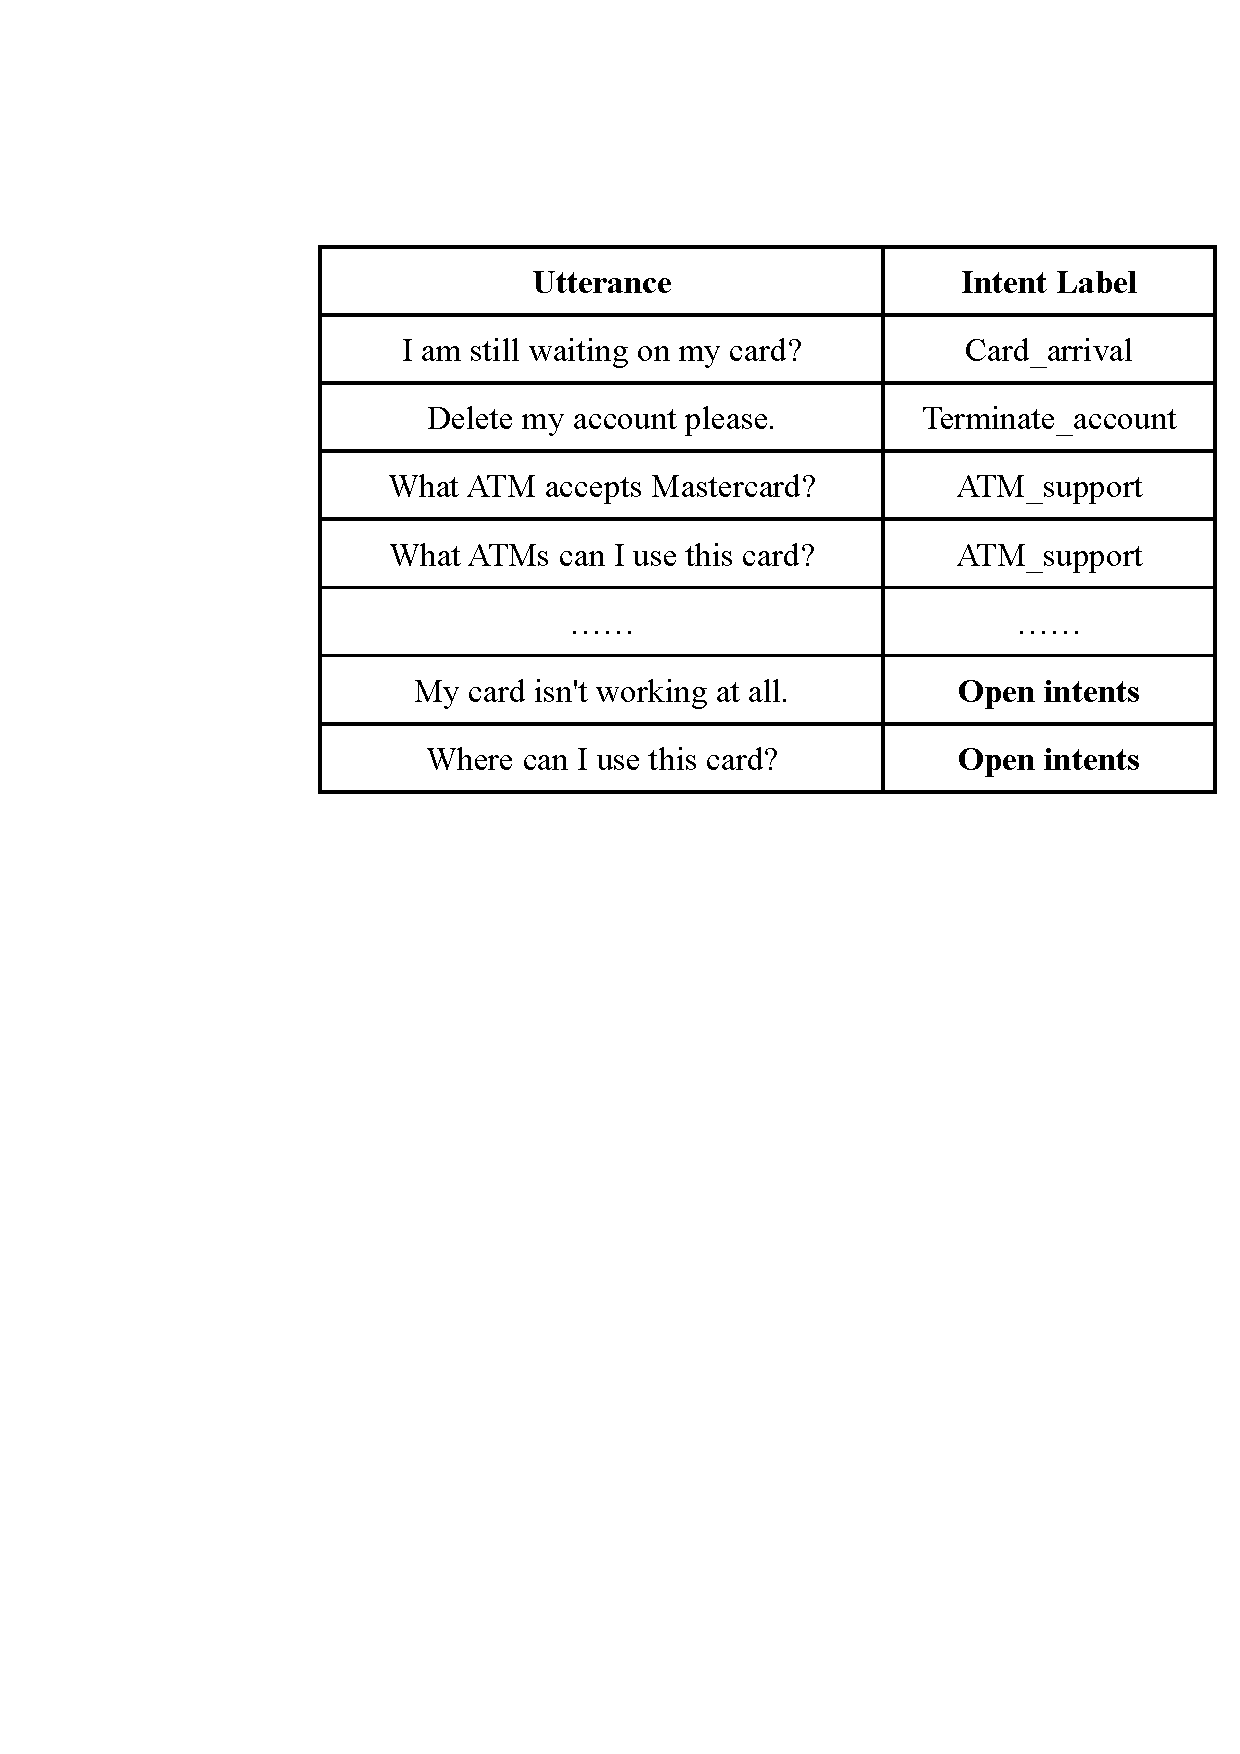
\includegraphics[width=0.8\columnwidth]{example.pdf}
\caption{An example of open intent classification in banking domain. Card\_arrival, Terminate\_account, and ATM\_support are three known intents. Other unsupported intents are treated as open intents.}  \label{fig:example}
\end{figure}


Generally, the task of open intent classification can be viewed as a (K+1)-class classification problem, where the first K classes represent K known intents and the (K+1)-th class represents open intents.
For this task, the main challenge is how to detect open intents without any training samples of open intents.
To address this challenge, recent studies mainly focused on designing outlier detection algorithms combined with K-class classifier.
In this kind of methods, as shown in the left part of Figure \ref{fig:motivation}, the open intents can be detected by judging whether the input sample is an outlier of all known intents.

Along this line of work, researchers mainly consider how to calibrate the decision boundary of each known intent class for outlier detection.
An intuitive solution is to simply use a threshold on the K-class classifier's prediction probability to decide whether a sample is an outlier of all known intents \cite{Shu17,DBLP:conf/emnlp/CavalinRAP20}.
However, since the deep learning methods tend to overfit the training samples, the K-class classifier would produce overconfident predictions of known intents \cite{DBLP:conf/iclr/LiangLS18,DBLP:conf/cvpr/Hein}.
Thus, even the sample of open intents would be easily classified with high probability into the K known intents, which makes the threshold hard to decide.
To this end, some subsequent work chooses to use more flexible outlier detection algorithms to calibrate the decision boundary.
For example, Lin et al. \cite{Lin19} and Yan et al. \cite{Yan20} propose to first learn discriminative deep features through large margin cosine loss and Gaussian mixture loss, and then apply the local outlier factor algorithm to detect open intents.
Xu et al. \cite{DBLP:conf/coling/XuHYLLX20} also proposes to first learn discriminative deep features through large margin cosine loss, and then apply Mahalanobis distance to detect open intents.
Considering the feature learning is optimized separately from decision boundary learning in these methods, Zhang et al. \cite{zhang21} proposes a joint optimized adaptive decision boundary method for outlier detection.

\begin{figure}[t]
\centering
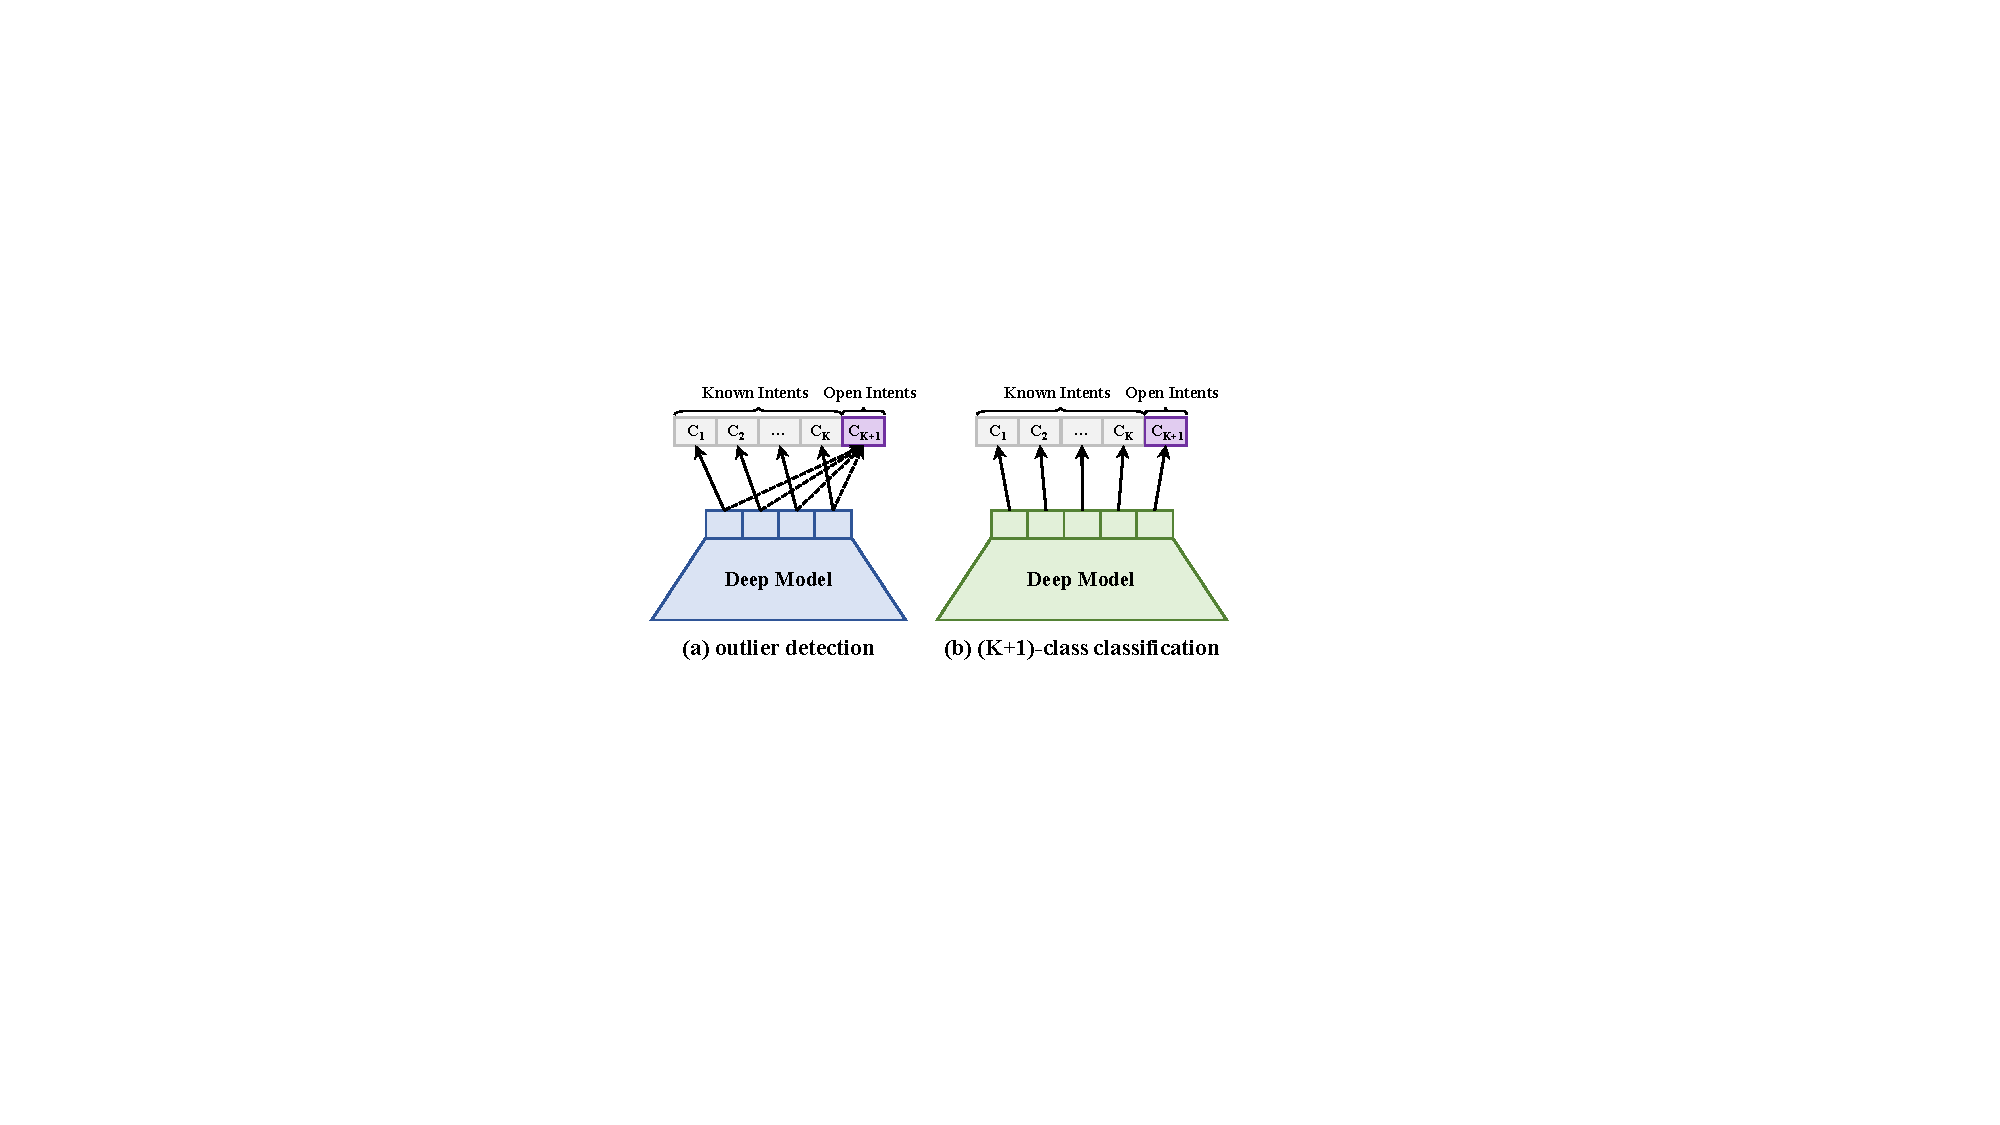
\includegraphics[width=1\columnwidth]{Illustration.pdf}
\caption{Illustration of two kinds of deep open intent classification models. The left part is the idea of existing methods and the right part is our method.}
\label{fig:motivation}
\end{figure}


\iffalse
\begin{figure*}
  \centering
  \subfigure[Illustration of two kinds of deep open intent classification models. The left part is the idea of existing methods and the right part is our method.]{
        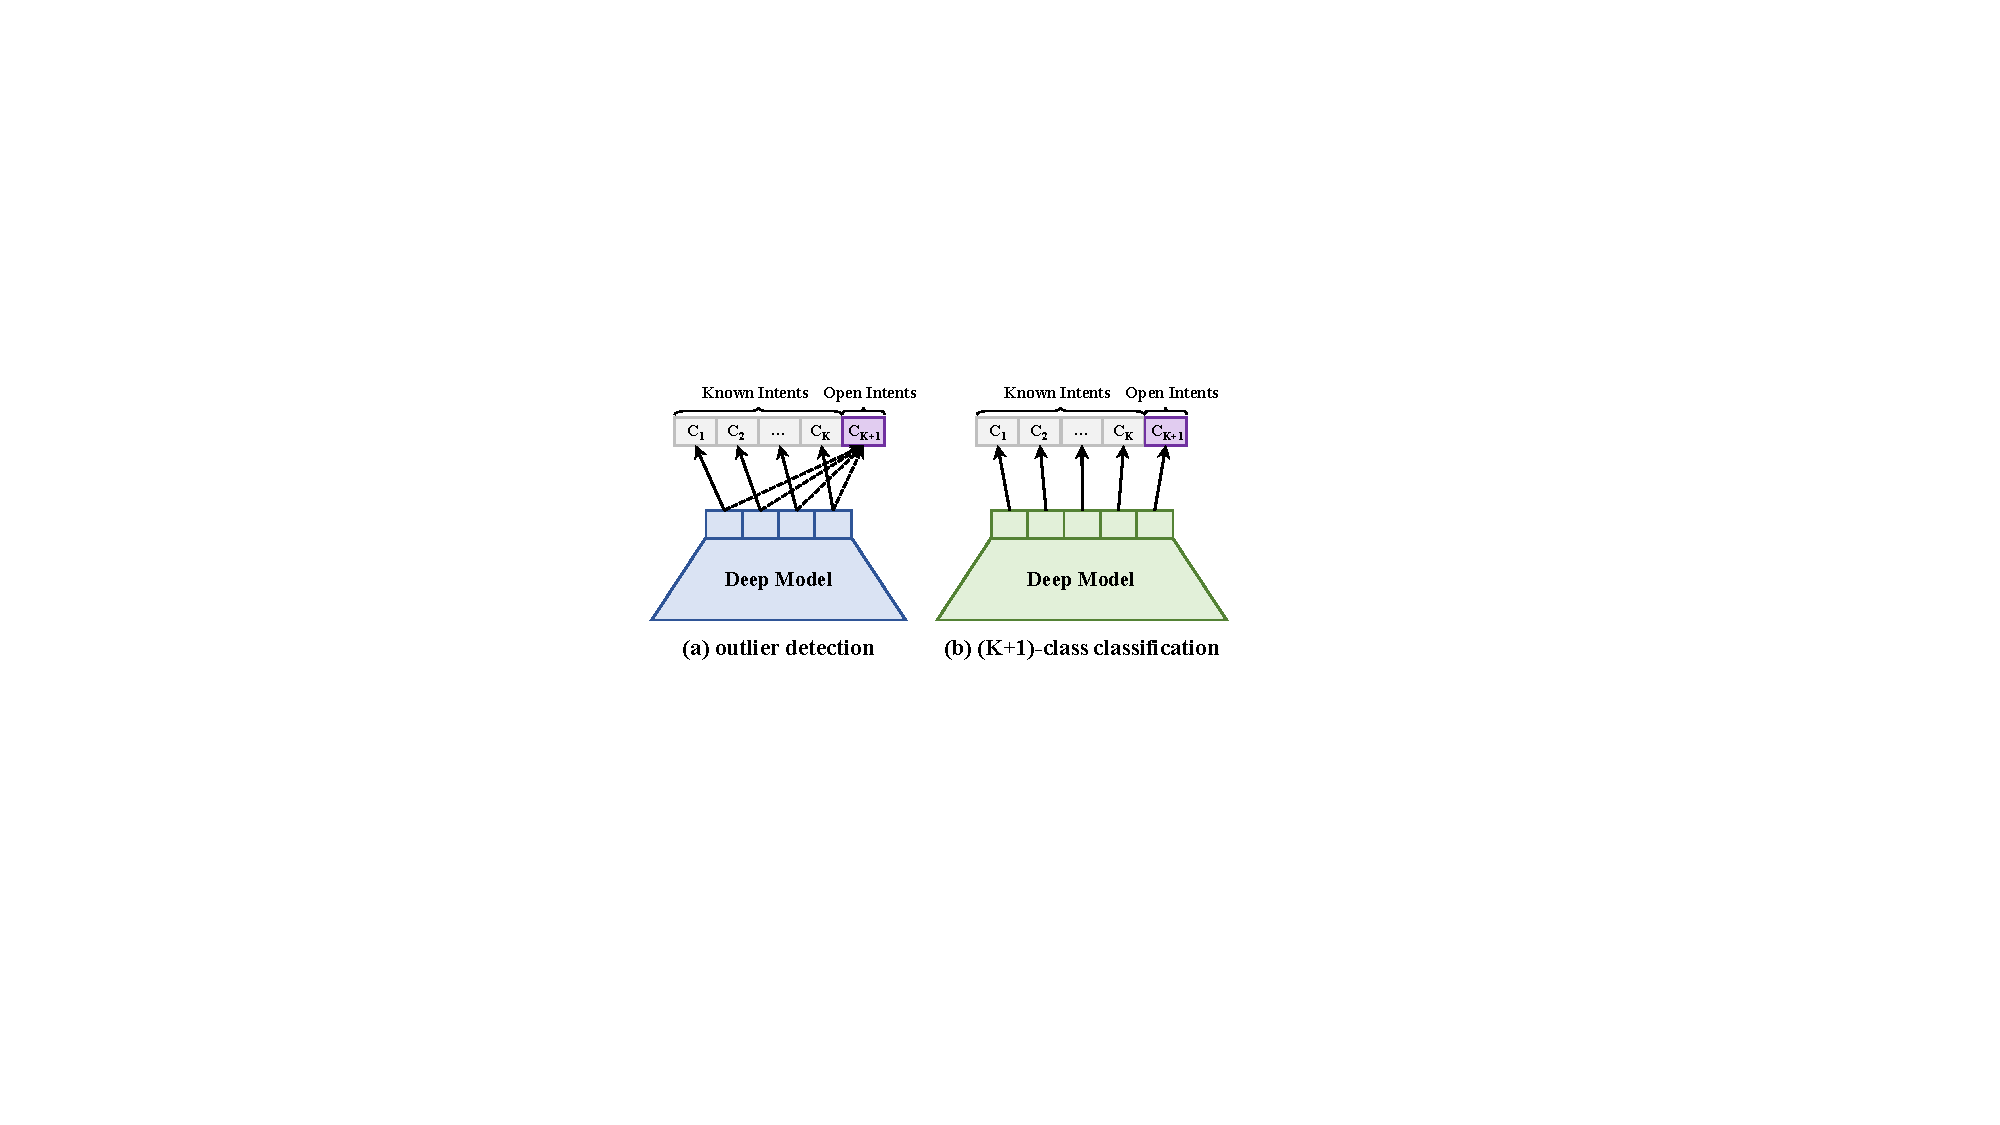
\includegraphics [width=0.4 \textwidth]{Illustration.pdf}
        }\label{fig:motivation}
        \subfigure[An example of open intent classification in banking domain. Card\_arrival, Terminate\_account, and ATM\_support are three known intents. We should identify them correctly while detecting out-of-scope intent.]{
 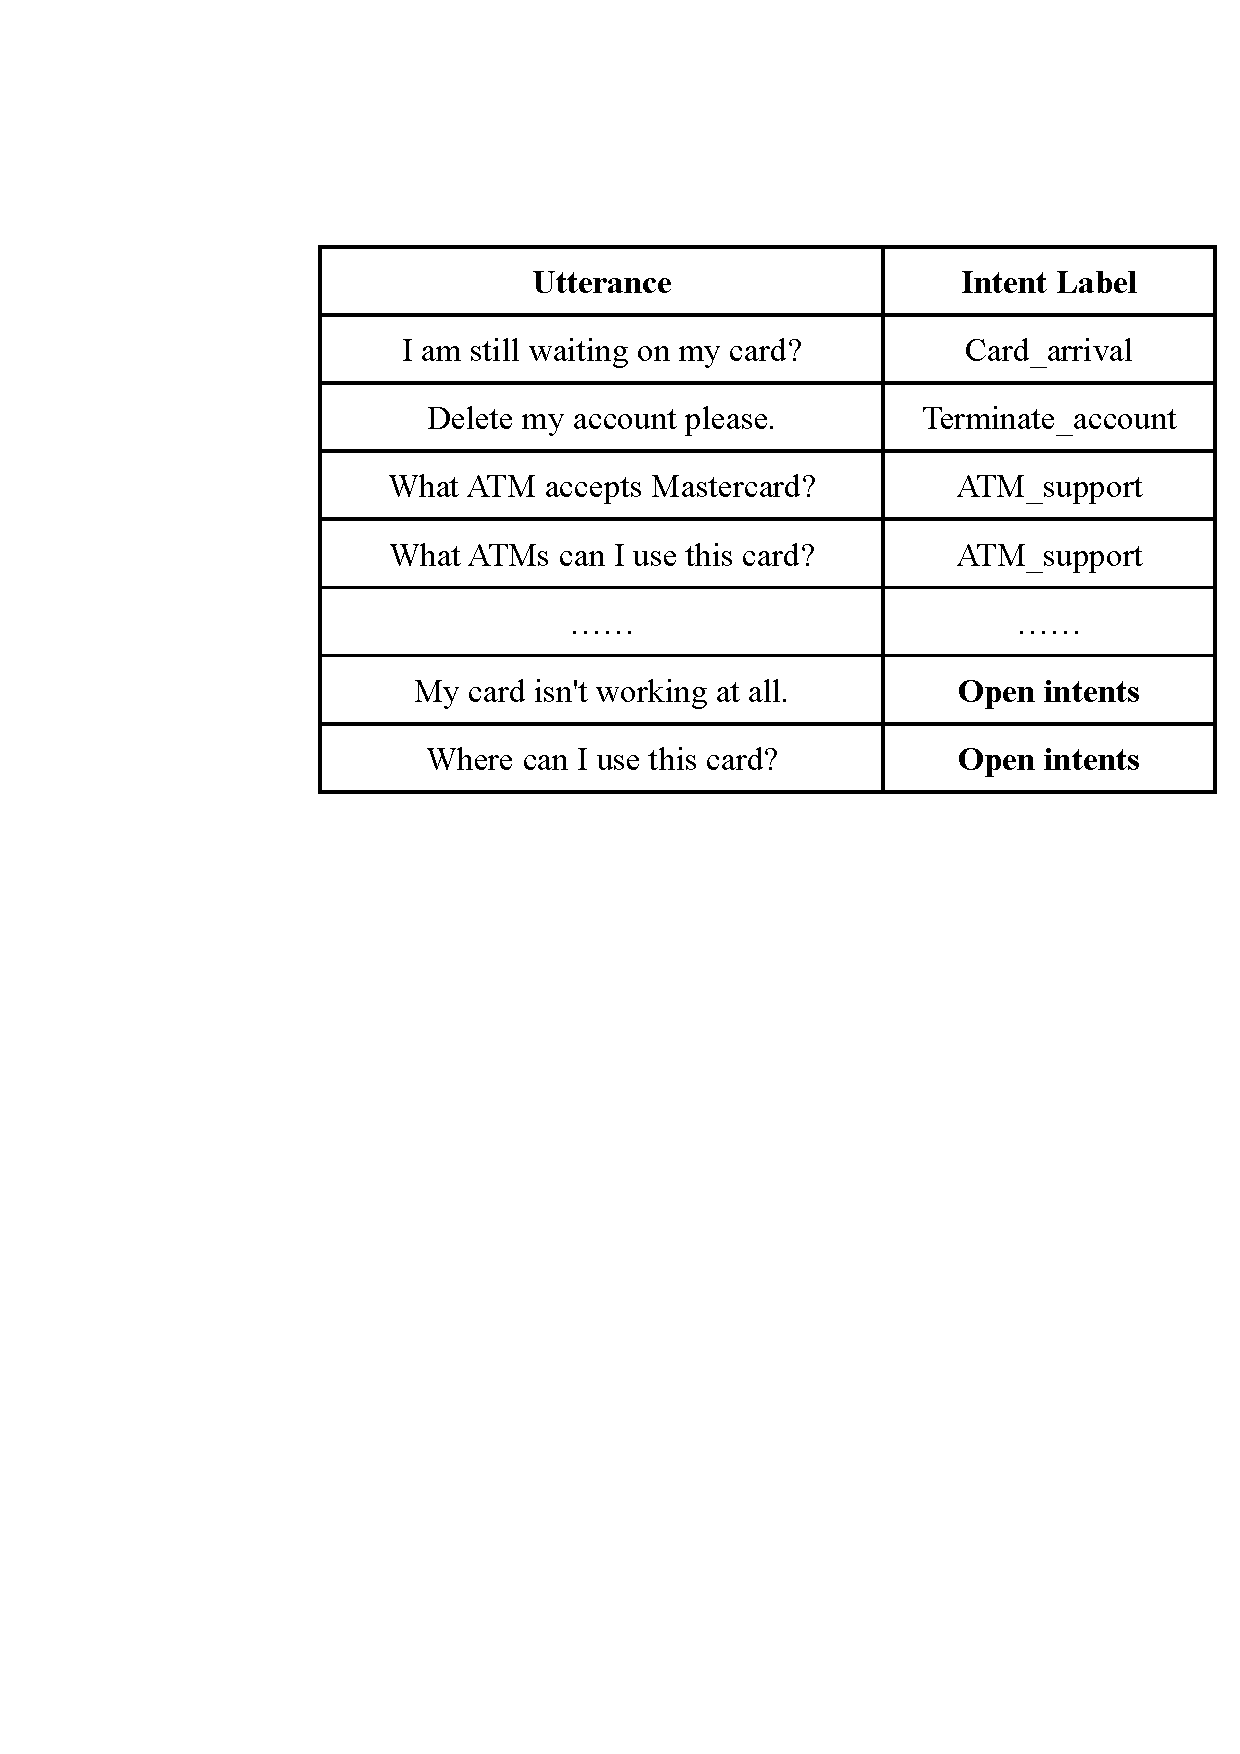
\includegraphics [width=0.4 \textwidth]{example.pdf}
  }
  %\vspace{-0.8em}
  \caption{Effect of local context window} \label{window}
\end{figure*}
\fi

In this paper, we consider another way without using outlier detection algorithms.
As shown in the right part of Figure \ref{fig:motivation}, instead of combining K-class classifier with outlier detection algorithms, we directly train a (K+1)-class classifier for open intent classification.
Training a (K+1)-class classifier with training samples of only K classes is very challenging.
Obviously, there are two main challenges: one is how to calibrate the decision boundary of the K known intent classes to avoid the overconfident prediction on known intents, and the other is how to learn the decision boundary of the (K+1)-th open intent class to enable test samples to be classified as open intents.
For the first challenge, our intuition is whether we can reshape the label distribution of training samples of known intents to reduce overconfident prediction on known intents.
For the second challenge, our intuition is whether we can generate some pseudo samples for open intents based on existing training samples to optimize the decision boundary of open intents.

To this end, we propose a deep open intent classification model based on Soft Labeling and Manifold Mixup (SLMM).
Specifically, for the overconfident prediction problem, we design a Soft Labeling (SL) strategy to reshape the label distribution of training samples, which reallocates the probability of the known intent samples on the class of known intents to the class of open intents.
Soft labeling allows the model to give each sample a probability of being predicted as an open intent, thus reducing overconfident prediction on known intents.
For the optimization problem of open intents, we design a Manifold Mixup (MM) strategy to generate pseudo samples for open intents, which interpolates the representation of two samples of different known intents.
While the interpolation between two different known intents can be regarded as a low-confidence area of both known intents, we use the samples in these low-confidence areas as pseudo open intent samples to learn the decision boundary of open intents.
Based on these two strategies, our model can be trained with label-reshaped samples of known intents and pseudo samples of open intents, and thus can be effectively used for open intent classification.

The major contributions of this paper are summarized as follows:
\begin{itemize}
\item We propose a (K+1)-class classification framework for the task of open intent classification without using outlier detection algorithms.
\item We propose two strategies (i.e., soft labeling and manifold mixup) to learn decision boundary without using any additional data.
\item We conduct experiments on four benchmark datasets and the experimental results demonstrate that our model SLMM outperforms previous methods and achieves state-of-the-art performance.
\end{itemize}

\iffalse
The rest of this paper is organized as follows.
Section II introduces the related work of open intent classification and mixup, and highlights the differences between our proposed model and previous work.
Section III gives the definition of open intent classification task and elaborates on our proposed
approach, including soft labeling and manifold mixup, as well as how to integrate them.
Section IV reports the evaluation results of the proposed method against baselines and conducts comprehensive experiments for analysis.
Section V summarizes this work.
\fi

\begin{figure*}[t]
\centering
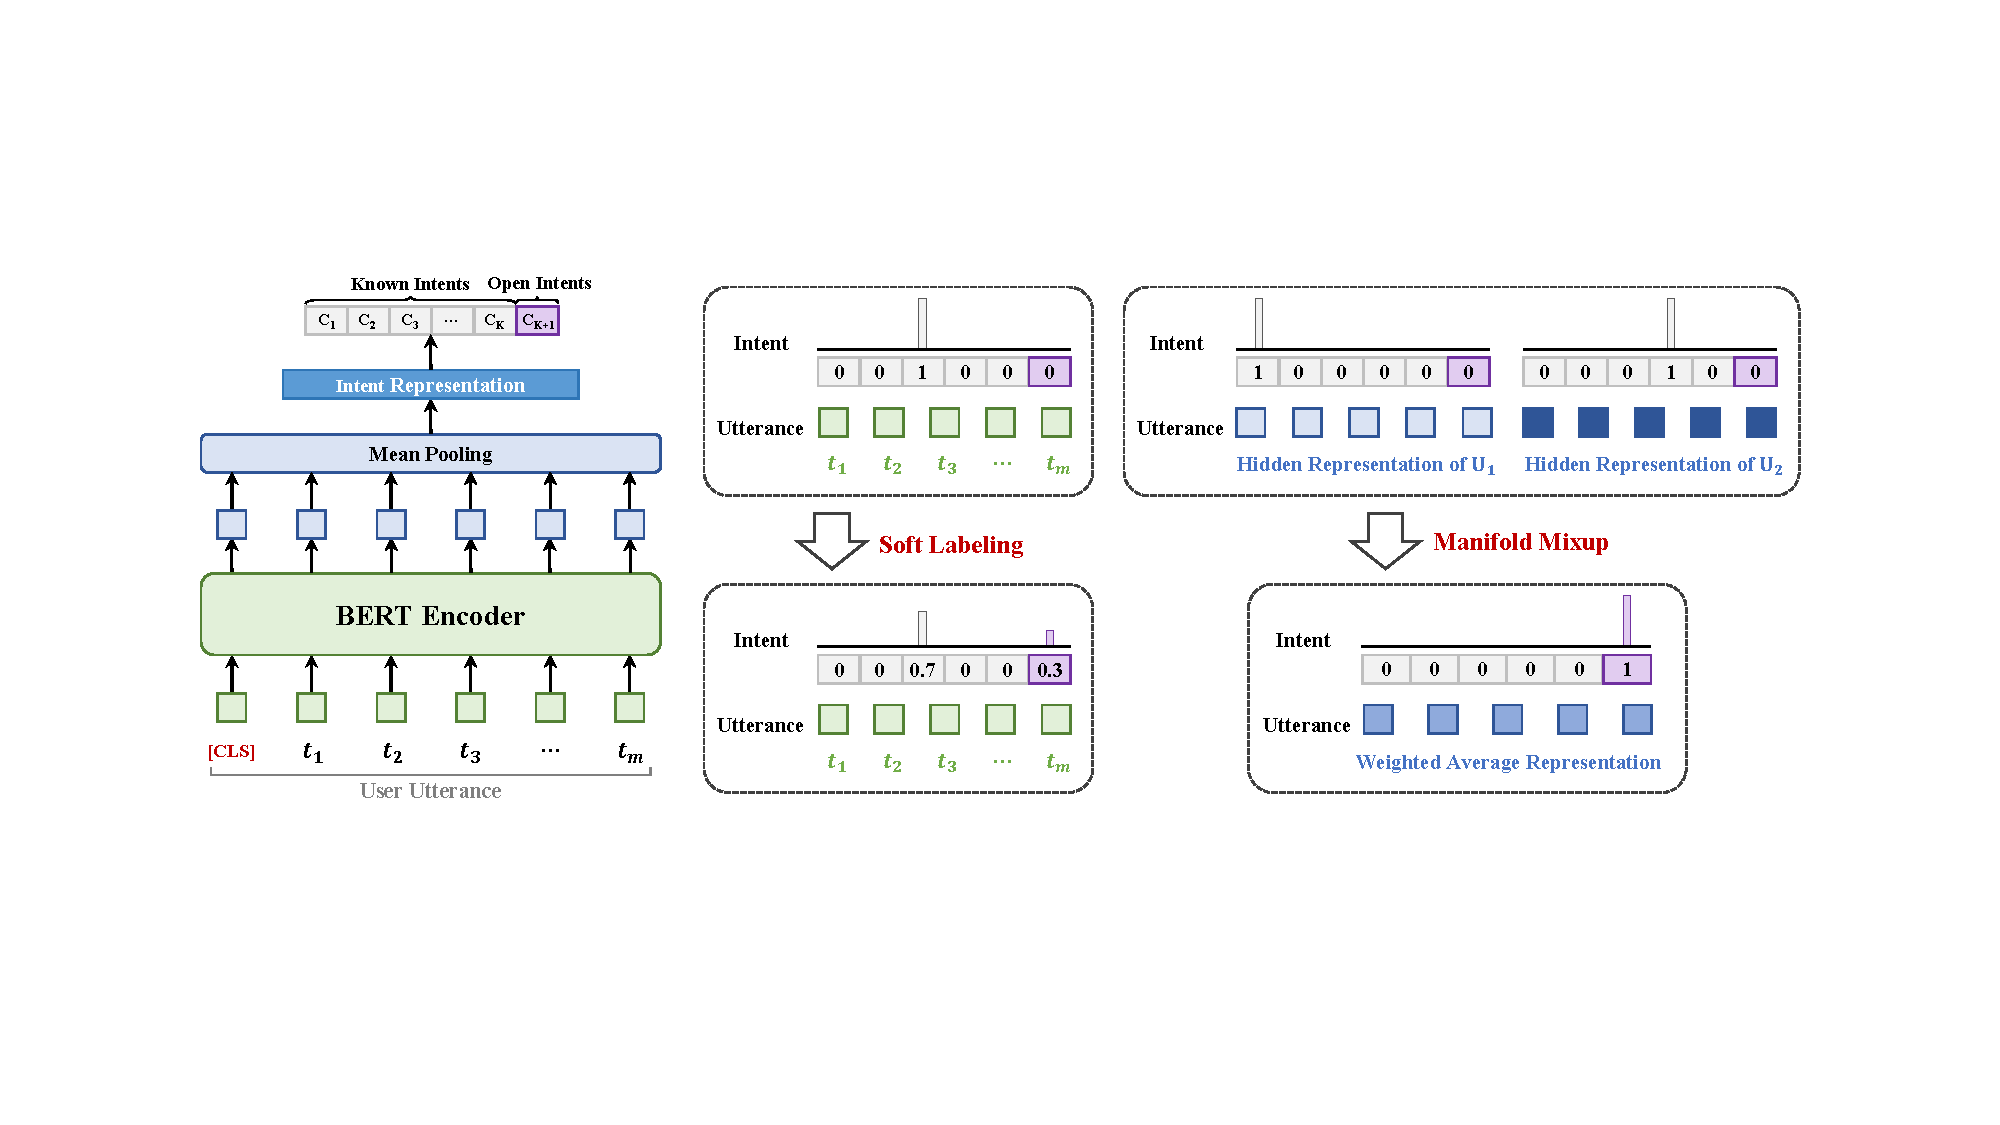
\includegraphics[width=2\columnwidth]{Framework.pdf}
\caption{Framework of our proposed method. The left part is model backbone in our proposed method. The middle part is soft labeling strategy and the right part is manifold mixup strategy.}
\label{fig:model}
\end{figure*}


\section{Related Work}
In this section, we introduce the following two research topics relevant to our work.

\subsection{Open Intent Classification}
Intent detection is an important component of dialogue system.
Many methods have been proposed to solve this task in recent years \cite{DBLP:conf/emnlp/LiLQ18,DBLP:conf/acl/ENCS19,DBLP:conf/emnlp/QinCLWL19,DBLP:conf/acl/ZhangLDFY19,Qin21} and most of these methods work well with the $closed$-$world$ assumption.
However, such an assumption is commonly violated in practical systems that are deployed in a dynamic or open environment.
Practical systems often encounter queries that fall outside their supported intents.
Therefore, recognizing queries that fall outside supported intents has gained attention recently.

In the past few years, researchers have proposed various methods to deal with this open intent detection problem.
The first group of methods mainly focuses on the out-of-domain intent detection \cite{DBLP:conf/emnlp/RyuKYL18,Kim18,DBLP:conf/aaai/PodolskiyLBAP21,Xu21}.
This task can be formalized as a binary classification problem, which aims to distinguish between in-domain data and out-of-domain data and does not require the more fine-grained classification of known intents.

Unlike these methods, the second group of methods expects to be able to detect the out-of-domain intents while at the same time performing more fine-grained classification for known intents.
In these methods, some labeled open intents samples are available in training data~\cite{DBLP:conf/emnlp/LarsonMPCLHKLLT19,DBLP:journals/taslp/ZhengCH20,DBLP:conf/naacl/ZengHYXX21}.
However, under open environment, collecting data of open intents is very difficult and expensive.
Thus, the third group of methods is proposed to focus on a more practical setting, which expects to train the open intent classification model without using any labeled samples of open intents in training data~\cite{Lin19,Yan20,DBLP:conf/emnlp/CavalinRAP20,DBLP:conf/coling/XuHYLLX20,zhang21,Tan19,Zhang20}.
Considering the scarcity of data in practice, Tan et al.~\cite{Tan19} and Zhang et al.~\cite{Zhang20} explore the few-shot scenario (i.e., the samples of known intents are few-shot).

Among the third group of methods, current methods mainly employ the outlier detection algorithms for open intent detection.
These methods can be further divided into three categories: threshold-based, post-processing, and joint-optimization.
The threshold-based methods simply use a threshold of prediction probability to judge whether the example belongs to open intents.
Cavalin et al. \cite{DBLP:conf/emnlp/CavalinRAP20} designs such a method, which is based on a special word graph and the threshold is applied to the maximum prediction probability of nodes in graph.
The post-processing methods first learn a feature space based on training samples of known intents and then apply the outlier detection algorithm on the feature space to detect open intents in a post-processing way.
Lin et al. \cite{Lin19} proposes a two-step method which uses large margin cosine loss (LMLC) to learn discriminative features and then uses a density-based detection algorithm LOF to detect open intents.
Yan et al. \cite{Yan20} proposes a semantic-enhanced Gaussian mixture model to learn discriminative features and also uses the LOF algorithm to detect open intents.
Xu et al. \cite{DBLP:conf/coling/XuHYLLX20} proposes BiLSTM with LMLC as a feature extractor and uses Gaussian discriminant analysis (GDA) and Mahalanobis distance to detect open intents.
%Zeng et al. \cite{DBLP:conf/naacl/ZengHYXX21} proposes a contrastive learning framework to model discriminative feature and also uses GDA and Mahalanobis distance to detect open intents.
Similar to the post-processing methods, the joint-optimization methods also detect open intents in a post-processing way, but they consider to jointly learn the feature space and the decision boundary of outlier detection.
Zhang et al. \cite{zhang21} proposes a joint optimized adaptive decision boundary method for open intent classification.

\iffalse
\subsection{Out-Of-Domain Detection}
Out-of-domain detection is a binary classification problem and emphasizes that data comes from different domains.
Many work focuses on out-of-domain intent detection \cite{DBLP:conf/emnlp/RyuKYL18,Kim18}.
And open classification also requires accurate classification of known classes \cite{DBLP:journals/geng}.
\fi


\iffalse
\subsection{Open World Classification}

Most of existing classification models are built by the $closed$-$world$ assumption.
However, such an assumption is commonly violated in practical systems that are deployed in a dynamic or open environment.

Various methods have been proposed to improve the performance of open world classification.
Early work in this field primarily focused on SVM based approaches \cite{DBLP:conf/nips/ScholkopfWSSP99,DBLP:journals/pami/ScheirerRSB13,DBLP:conf/eccv/JainSB14,DBLP:journals/pami/ScheirerJB14}.
Recently, many deep neural network models are proposed for open world classification.
Most of them follow a threshold-based method \cite{DBLP:conf/naacl/Fei016,Hendrycks17,Shu17,DBLP:conf/iclr/LiangLS18}.
The samples whose scores are lower than the threshold are considered to be rejected.
\fi

\subsection{Mixup}
Mixup \cite{ZhangCDL18} is a recent proposed data augmentation method, which can construct virtual samples by linear interpolation between two random samples.
As a special mixup method, manifold mixup \cite{DBLP:conf/icml/VermaLBNMLB19} is also able to construct virtual samples, but its specialness is that it constructs samples by interpolating the hidden representation of samples.
Since manifold mixup often leads to smoother decision boundaries that are further away from the training data, it is usually used to improve the generalization of neural network.
While these mixup methods are mainly adopted in the field of computer vision, recently, some work has tried to use them in the field of natural language processing \cite{DBLP:conf/acl/ChengJME20,DBLP:conf/acl/ChenYY20,DBLP:conf/emnlp/ZhangYZ20,DBLP:conf/emnlp/ChenWTYY20,DBLP:conf/www/MiaoLWT20}.
Among them, Cheng et al. \cite{DBLP:conf/acl/ChengJME20} performs interpolations at the embedding space in sequence-to-sequence learning for machine translation.
Chen et al. \cite{DBLP:conf/acl/ChenYY20} and Miao et al. \cite{DBLP:conf/www/MiaoLWT20} explore mixup on semi-supervised text classification task.
Chen et al. \cite{DBLP:conf/emnlp/ChenWTYY20} and Zhang et al. \cite{DBLP:conf/emnlp/ZhangYZ20} explore interpolation on sequence labeling tasks.
Different from most previous studies that use mixup methods to augment data and improve model generalization, we adopt manifold mixup in the task of open intent classification and mainly use it to generate samples for previous unseen intents.
In the same period of our work, some work \cite{DBLP:conf/cvpr/ZhouYZ21,DBLP:conf/acl/ZhanLLFWL21} use mixup to generate data for open class and model this task as (K+1)-class classification.
Zhou et al. \cite{DBLP:conf/cvpr/ZhouYZ21} learns placeholders for open-set recognition, consisting of classifier placeholder and data placeholder.
They use adaptive threshold to learn classifier placeholder and use mixup to learn data placeholder.
Zhan et al. \cite{DBLP:conf/acl/ZhanLLFWL21} constructs two types of pseudo outliers by using mixup and leveraging publicly available auxiliary datasets to form a consistent (K+1)-class classification task.

\section{Method}
In this section, we first present the task definition of open intent classification.
Then we introduce the overview of our proposed method and the detailed model architecture.
Finally, we detail the training and inference process of the method. 
\subsection{Task Definition}
We first introduce some notation and formalize the open intent classification task.
Let $\mathcal{D}_{tr} = \{(x_i,y_i)\}_{i=1}^{L}$ denote the training set, where $x_i$ is a training utterance (sample), $y_i \in Y = \{1,2,\cdots,K\}$ is the ground-truth intent (label) of $x_i$, and $L$ is the number of utterances in the training set.
Let $\mathcal{D}_{te} = \{(x_j,y_j)\}_{j=1}^{U}$ denote a test set, where $x_j$ is a test utterance, $y_j \in \hat{Y} = \{1,2,\cdots,K,K+1\}$ is the ground-truth intent of $x_j$, and $U$ is the number of utterances in the test set.
Note that the class $K+1$ in $\hat{Y}$ is a proxy class for open intents which has not been seen in the training set $\mathcal{D}_{tr}$.
Then, the goal of open intent classification is to learn a model based on the training set $\mathcal{D}_{tr}$ and apply it on the test set $\mathcal{D}_{te}$ to (1) predict the correct intents for utterances of known intents, and (2) identify utterances of open intents.
\iffalse
Then, the goal of open intent classification is to learn a function $F$ based on the training set $\mathcal{D}_{tr}$ and apply it on the test set $\mathcal{D}_{te}$ to (1) predict the correct intents for utterances of known intents, and (2) identify utterances of open intents, by
\begin{equation}\label{eq:formulation}
  \hat{y}=F(x;\theta^*=\theta^*(\mathcal{D}_{tr})).
\end{equation}
where $\theta^*$ is a sufficient statistic learned for prediction $p_{\theta^*}(y|x)$ based on the labeled data $\mathcal{D}_{tr}$.
\fi

\subsection{An Overview of SLMM}
As shown in the left part of Figure \ref{fig:model}, our model takes user utterance as input and conducts (K+1)-class classification to predict the corresponding class directly.
The training of our model consists of two stages: pre-training for known intents and training for open intents.
We first pre-train the model based on the labeled samples of known intents to get better intent representation.
Then we propose two strategies for training open intents, named soft labeling and manifold mixup, as shown in the middle and right part of Figure \ref{fig:model}.
Finally, our model can be directly used for inference.


\subsection{Deep Open Intent Classification Model}
We then introduce the architecture of our deep open intent classification model.
As shown in the left part of Figure \ref{fig:model}, we use BERT \cite{Devlin19} as model backbone to extract intent representation.
Given the $i$-th user utterance $x_i = \{t_1,t_2,\cdots,t_{m_i}\}$, we can get all token embeddings $[CLS,T_1,\cdots,T_{m_i}] \in \mathbb{R}^{({m_i}+1) \times H}$ from the last hidden layer of BERT, where $CLS$ is the token embedding of a special token, $m_i$ is the sentence length of the $i$-th user utterance, and $H$ is the hidden layer size.
Same as previous work \cite{Lin20,zhang21}, we apply the mean pooling layer on the token embeddings to get the averaged representation $\tilde{x}_i \in \mathbb{R}^H$:
\begin{equation}
    \tilde{x}_i = \text{mean-pooling}([CLS,T_1,\cdots,T_{m_i}])
\end{equation}

After that, we further strengthen feature extraction capability by feeding $\tilde{x}_i$ to a dense layer $h$ to get the intent representation $z_i \in \mathbb{R}^D$:
\begin{equation}
    z_i = h(x_i) = {\rm ReLU}(W_hx_i+b_h)
\end{equation}
where $D$ is the dimension of the intent representation, $W_h \in \mathbb{R}^{H \times D}$ and $b_h \in \mathbb{R}^{D}$ denote the weight and bias term of layer $h$ respectively.


\subsection{Pre-training for Known Intents}
To get better intent representation for open intent classification, we first pre-train the model based on the labeled data of known intents in training set $\mathcal{D}_{tr}$.
The intent representation $z_i$ can be learned with the softmax loss $\mathcal{L}_P$:
\begin{equation}
    \mathcal{L}_P = -\frac{1}{L} \sum_{i=1}^L {\rm log} \frac{{\rm exp}(\phi_K(z_i)^{y_i})}{\sum_{j=1}^K {\rm exp}(\phi_K(z_i)^j)}
\end{equation}
where $L$ is the size of training set, $\phi_K(\cdot)$ is a K-class classifier, and $\phi_K(\cdot)^j$ is the output logits of the $j$-th class.
Note that the classifier $\phi_K(\cdot)$ is a subset of $\phi_{K+1}(\cdot)$ and is corresponding to the classifier of the known intents part.

\subsection{Training for Open Intents}
Due to the lack of training data specific to open intents, training the model for the detection of open intents is challenging. 
To this end, we propose two strategies to generate pseudo data for the further training of model, which are soft labeling and manifold mixup.
Among these two strategies, soft labeling generate pseudo data for known intents by reshaping the label distribution of samples in training set.
Manifold mixup generates pseudo data for open intents by interpolating between the intent representations of two samples with different known intents. 

\subsubsection{Soft Labeling}

For the soft labeling strategy, our intuition is that if each training sample has a certain probability to be classified as open intents, model's overconfidence prediction on known intents would be reduced and the outlier samples of all known intents would be easier to be detected as open intents.
Thus, instead of using the one-hot label distribution, we soften the label distribution of each sample in training set by reallocating part of its probability on the class of known intents to the class of open intents.

In detail, as shown in the middle part of Figure \ref{fig:model}, for each known intent sample, we can perform soft labeling by setting the probability on open intent class as a default value $\xi$ and the probability on its ground-truth intent class as $1-\xi$.
It is worth noting that we usually set a small probability to the open class (e.g., 0.3), so that the probability of ground-truth class can be higher than that of open class.
This allows the model to have the ability of identifying open intent while at the same time avoiding the model overfitting to the open intent class.
After that, we can train the model on these pseudo samples with soft labeling via a KL-divergence loss:
 \begin{equation}
    \mathcal{L}_S = \sum_{i=1}^{L}D_{KL}\left(p(x_i)||q(x_i)\right)
\end{equation}
where $L$ is the size of training set, $p(x_i)$ is the softened probability distribution (generated by soft labeling) of the utterance $x_i$ on all intents, $q(x_i)$ is the output probability distribution of applying softmax on $\phi_{K+1}(z_i)$, and $z_i$ is the intent representation of the utterance $x_i$.

\begin{algorithm}[t]
\caption{Training Flow of SLMM}
\label{alg:inference}
\begin{algorithmic}[1]
\REQUIRE The training set
\ENSURE A open intent classification model.
\STATE \textbf{\emph{\# Pre-training for Known Intents:}}
\FORALL{iteration = 1, $\cdots$, MaxIter}
\STATE Sample a mini-batch $\{(x_i,y_i)\}$
\STATE Calculate the training loss by Eq. (3)
\STATE Obtain derivative and update the model
\ENDFOR
\STATE \textbf{\emph{\# Training for Open Intents:}}
\FORALL{iteration = 1, $\cdots$, MaxIter}
\STATE Sample a mini-batch $\{(x_i,y_i)\}$
\STATE Reshape label distribution via soft labeling
\STATE Calculate soft labeling loss by Eq. (4)
\STATE Generate pseudo data via manifold mixup
\STATE Calculate manifold mixup loss by Eq. (8)
\STATE Calculate total loss by Eq. (9)
\STATE Obtain derivative and update the model
\ENDFOR
\RETURN The model converges on validation set.
\end{algorithmic}
\end{algorithm}

\begin{table*} \setlength{\tabcolsep}{15pt}
\centering
\caption{Statistics of dataset.}\label{statis}
\begin{tabular}{lcccccc}
\toprule
\textbf{Dataset}&\textbf{Classes}&\textbf{\#Training}&\textbf{\#Validation}&\textbf{\#Test}&\textbf{Vocabulary Size}&\textbf{Length(mean)} \\
\midrule
\textbf{BAKING} & 77 &9003&1000&3080&5028&11.91  \\
\textbf{CLINC} & 150 &15000&3000&5700&8376&8.31  \\
%\textbf{StackOverflow} & 20 & 12000&2000&6000&17182&9.18   \\
\textbf{SNIPS} & 7 & 13084 & 700 & 700 & 11971& 9.05   \\
\textbf{ATIS} & 18 & 4978 & 500 & 893 & 938 & 11.37 \\
\bottomrule
\end{tabular}
\end{table*}

\subsubsection{Manifold Mixup}
For the manifold mixup strategy, our intuition is that if the outlier samples of known intents can be used as open intent samples for model training, the decision boundary between known intents and open intents could be better learned.
To this end, we propose to apply manifold mixup to generate open intent samples by interpolating between the representation of two samples of different known intents.
%Our assumption is that the interpolated representation can be viewed as the outlier of the corresponding known intents before interpolation.
Our assumption is that the interpolated representation can be viewed as the sample of open intents.

In detail, as shown in the right part of Figure \ref{fig:model}, given two samples from different known intents, we can perform manifold mixup by interpolating their output of the $n$-th layer of BERT and labeling the interpolated representation as open intent.
Specifically, given a batch of known intent samples, we randomly select sample pairs for manifold mixup by random shuffling.
By recording the list of samples before and after random shuffling, samples at the same position in these two lists can realize random pairing.
For each sample pair $(x_i,x_j)$, if they are from different known intents (i.e., from different classes), we feed them into BERT, and get their representations until reaching $n$-th layer by:
\begin{equation}
\begin{aligned}
    h_i^l = {\rm BERT}(h_{i}^{l-1}), l\in[1,n]\\
    h_j^l = {\rm BERT}(h_{j}^{l-1}), l\in[1,n]
\end{aligned}
\end{equation}
where $h_i^l$ and $h_j^l$ are the hidden representation of sample pair $(x_i,x_j)$ after the $l$-th layer.
Then we mix the two hidden representations and continue forwarding:

\begin{equation}
    \hat{h}_m^n = \lambda h_i^n + (1-\lambda)h_j^n
\end{equation}
\begin{equation}
    \hat{h}_m^l = {\rm BERT}(\hat{h}_m^{l-1}), l\in[n+1,T]
\end{equation}
where $T$ is total number of layers in BERT, $\lambda \in$ [0,1] is a value sampled from Beta ($\alpha$,$\alpha$) distribution.
After getting the output $\hat{h}_m^T$ from BERT, we use mean-pooling and dense layer $h$ to get the intent representation $\hat{z}_m$.
The intent representation $\hat{z}_m$ is then fed into the classifier $\phi_{K+1}(\cdot)$ for open intent classification and the softmax loss is:
\begin{equation}
    \mathcal{L}_M = -\frac{1}{M} \sum_{m=1}^M {\rm log} \frac{{\rm exp}(\phi_{K+1}(\hat{z}_m)^{K+1})}{\sum_{k=1}^{K+1} {\rm exp}(\phi_{K+1}(\hat{z}_m)^k)}
\end{equation}
where and $M$ is the number of pseudo samples of open intents generated by manifold mixup, $\phi_{K+1}(\cdot)$ is the (K+1)-class linear classifier, and $\phi_{K+1}(\cdot)^k$ is the output logits of the $k$-th class.

\iffalse
%std
\begin{table*}[t]\small  \setlength{\tabcolsep}{3pt}
  \centering
  \caption{\textcolor{blue}{Performance of open intent classification with different known class ratios (25\%, 50\%, 75\%) on four benchmark datasets. “Accuracy” and “F1” denote the accuracy score and macro F1-score over all classes. Performance (mean$\pm{\text{std}}$) over 10 runs are reported. The best results are in bold. All results of baselines on BANKING and CLINC from Zhang et al. \cite{zhang21}. The results of ADB on SNIPS and ATIS are reproduced from open-source code.}}  \label{tab:performance_comparison}
    \begin{tabular}{cccccccccccc}
    \toprule
    &\multirow{2}{*}{\textbf{Methods}}&\multicolumn{2}{c}{\textbf{BANKING}}&\multicolumn{2}{c}{\textbf{CLINC}}&\multicolumn{2}{c}{\textbf{SNIPS}}&\multicolumn{2}{c}{\textbf{ATIS}}\\
    \cmidrule(lr){3-4} \cmidrule(lr){5-6} \cmidrule(lr){7-8}\cmidrule(lr){9-10} 
    &&\textbf{Accuracy}&\textbf{F1}&\textbf{Accuracy}&\textbf{F1}&\textbf{Accuracy}&\textbf{F1}&\textbf{Accuracy}&\textbf{F1}\\
    \midrule
    \multirow{6}{1cm}{\tabincell{c}{\textbf{25\%}}}&
    \textbf{MSP}&43.67&50.09&47.02&47.62&-&-&-&-\\
    &\textbf{DOC}&56.99&58.03&74.97&66.37&-&-&-&-\\
    &\textbf{OpenMax}&49.94&54.14&68.50&61.99&-&-&-&-\\
    &\textbf{LMLC}&64.21&61.36&81.43&71.16&-&-&-&-\\
    %&\textbf{ADB}&78.85$\pm{2.52}$&71.62$\pm{1.14}$&87.59$\pm{0.58}$&77.19$\pm{0.15}$&67.41$\pm{3.22}$&69.89$\pm{2.67}$&63.90$\pm{14.90}$&53.21$\pm{8.64}$\\
    &\textbf{ADB}&78.85&71.62&87.59&77.19&67.41&69.89&63.90&53.21&\\
    &\textbf{SLMM}&\textcolor{blue}{\bf{80.96$\pm{\bf{0.83}}$}}&\textcolor{blue}{\bf{72.58$\pm{\bf{0.79}}$}}&\textcolor{blue}{\bf{91.25$\pm{\bf{0.25}}$}}&\textcolor{blue}{\bf{80.04$\pm{\bf{1.22}}$}}&\textcolor{blue}{\bf{75.30$\pm{\bf{4.72}}$}}&\textcolor{blue}{\bf{74.64$\pm{\bf{3.48}}$}}&\textcolor{blue}{\bf{69.90$\pm{\bf{10.81}}$}}&\textcolor{blue}{\bf{61.18$\pm{\bf{9.44}}$}}\\
    \midrule
    \midrule
    \multirow{6}{1cm}{\tabincell{c}{\textbf{50\%}}}&
    \textbf{MSP}&59.73&71.18&62.96&70.41&-&-&-&-\\
    &\textbf{DOC}&64.81&73.12&77.16&78.26&-&-&-&-\\
    &\textbf{OpenMax}&65.31&74.24&80.11&80.56&-&-&-&-\\
    &\textbf{LMLC}&72.73&77.53&83.35&82.16&-&-&-&-\\
    %&\textbf{ADB}&78.86$\pm{0.61}$&80.90$\pm{0.36}$&86.54$\pm{1.10}$&85.05$\pm{0.83}$&80.36$\pm{1.36}$&82.96$\pm{1.36}$&81.27$\pm{0.56}$&63.24$\pm{4.92}$\\
    &\textbf{ADB}&78.86&80.90&86.54&85.05&80.36&82.96&81.27&63.24\\
    &\textbf{SLMM}&\textcolor{blue}{\bf{80.28$\pm{\bf{0.57}}$}}&\textcolor{blue}{\bf{81.98$\pm{\bf{0.47}}$}}&\textcolor{blue}{\bf{89.04$\pm{\bf{0.27}}$}}&\textcolor{blue}{\bf{86.72$\pm{\bf{0.08}}$}}&\textcolor{blue}{\bf{80.93$\pm{\bf{0.08}}$}}&\textcolor{blue}{\bf{83.15$\pm{\bf{0.15}}$}}&\textcolor{blue}{\bf{87.37$\pm{\bf{2.69}}$}}&\textcolor{blue}{\bf{70.21$\pm{\bf{2.44}}$}}\\
    \midrule
    \midrule
    \multirow{6}{1cm}{\tabincell{c}{\textbf{75\%}}}&
    \textbf{MSP}&75.89&83.60&74.07&82.38&-&-&-&-\\
    &\textbf{DOC}&76.77&83.34&78.73&83.59&-&-&-&-\\
    &\textbf{OpenMax}&77.45&84.07&76.80&73.16&-&-&-&-\\
    &\textbf{LMLC}&78.52&84.31&83.71&86.23&-&-&-&-\\
    %&\textbf{ADB}&81.08$\pm{0.10}$&85.96$\pm{0.01}$&86.32$\pm{0.53}$&88.53$\pm{0.18}$&82.56$\pm{1.22}$&85.13$\pm{1.10}$&87.53$\pm{0.28}$&71.60$\pm{1.62}$\\
    &\textbf{ADB}&81.08&85.96&86.32&88.53&82.56&85.13&87.53&71.60\\
    &\textbf{SLMM}&\textcolor{blue}{\bf{82.18$\pm{\bf{1.42}}$}}&\textcolor{blue}{\bf{86.67$\pm{\bf{0.75}}$}}&\textcolor{blue}{\bf{88.88$\pm{\bf{0.49}}$}}&\textcolor{blue}{\bf{90.40$\pm{\bf{0.53}}$}}&\textcolor{blue}{\bf{85.37$\pm{\bf{0.14}}$}}&\textcolor{blue}{\bf{85.57$\pm{\bf{0.21}}$}}&\textcolor{blue}{\bf{94.33$\pm{\bf{0.56}}$}}&\textcolor{blue}{\bf{81.00$\pm{\bf{1.03}}$}}\\
    \bottomrule
    \end{tabular}
\end{table*}
\fi


%final version : no blue
\begin{table*}[t]\small  \setlength{\tabcolsep}{3pt}
  \centering
  \caption{Performance of open intent classification with different known class ratios (25\%, 50\%, 75\%) on four benchmark datasets. “Accuracy” and “F1” denote the accuracy score and macro F1-score over all classes. Performance (mean$\pm{\text{std}}$) over 10 runs are reported. The best results are in bold. All results of baselines on BANKING and CLINC from Zhang et al. \cite{zhang21}. The results of ADB on SNIPS and ATIS are reproduced from open-source code.}  \label{tab:performance_comparison}
    \begin{tabular}{cccccccccccc}
    \toprule
    &\multirow{2}{*}{\textbf{Methods}}&\multicolumn{2}{c}{\textbf{BANKING}}&\multicolumn{2}{c}{\textbf{CLINC}}&\multicolumn{2}{c}{\textbf{SNIPS}}&\multicolumn{2}{c}{\textbf{ATIS}}\\
    \cmidrule(lr){3-4} \cmidrule(lr){5-6} \cmidrule(lr){7-8}\cmidrule(lr){9-10} 
    &&\textbf{Accuracy}&\textbf{F1}&\textbf{Accuracy}&\textbf{F1}&\textbf{Accuracy}&\textbf{F1}&\textbf{Accuracy}&\textbf{F1}\\
    \midrule
    \multirow{6}{1cm}{\tabincell{c}{\textbf{25\%}}}&
    \textbf{MSP}&43.67&50.09&47.02&47.62&-&-&-&-\\
    &\textbf{DOC}&56.99&58.03&74.97&66.37&-&-&-&-\\
    &\textbf{OpenMax}&49.94&54.14&68.50&61.99&-&-&-&-\\
    &\textbf{LMLC}&64.21&61.36&81.43&71.16&-&-&-&-\\
    %&\textbf{ADB}&78.85$\pm{2.52}$&71.62$\pm{1.14}$&87.59$\pm{0.58}$&77.19$\pm{0.15}$&67.41$\pm{3.22}$&69.89$\pm{2.67}$&63.90$\pm{14.90}$&53.21$\pm{8.64}$\\
    &\textbf{ADB}&78.85&71.62&87.59&77.19&67.41&69.89&63.90&53.21&\\
    &\textbf{SLMM}&\bf{80.96$\pm{\bf{0.83}}$}&\bf{72.58$\pm{\bf{0.79}}$}&\bf{91.25$\pm{\bf{0.25}}$}&\bf{80.04$\pm{\bf{1.22}}$}&\bf{75.30$\pm{\bf{4.72}}$}&\bf{74.64$\pm{\bf{3.48}}$}&\bf{69.90$\pm{\bf{10.81}}$}&\bf{61.18$\pm{\bf{9.44}}$}\\
    \midrule
    \midrule
    \multirow{6}{1cm}{\tabincell{c}{\textbf{50\%}}}&
    \textbf{MSP}&59.73&71.18&62.96&70.41&-&-&-&-\\
    &\textbf{DOC}&64.81&73.12&77.16&78.26&-&-&-&-\\
    &\textbf{OpenMax}&65.31&74.24&80.11&80.56&-&-&-&-\\
    &\textbf{LMLC}&72.73&77.53&83.35&82.16&-&-&-&-\\
    %&\textbf{ADB}&78.86$\pm{0.61}$&80.90$\pm{0.36}$&86.54$\pm{1.10}$&85.05$\pm{0.83}$&80.36$\pm{1.36}$&82.96$\pm{1.36}$&81.27$\pm{0.56}$&63.24$\pm{4.92}$\\
    &\textbf{ADB}&78.86&80.90&86.54&85.05&80.36&82.96&81.27&63.24\\
    &\textbf{SLMM}&\bf{80.28$\pm{\bf{0.57}}$}&\bf{81.98$\pm{\bf{0.47}}$}&\bf{89.04$\pm{\bf{0.27}}$}&\bf{86.72$\pm{\bf{0.08}}$}&\bf{80.93$\pm{\bf{0.08}}$}&\bf{83.15$\pm{\bf{0.15}}$}&\bf{87.37$\pm{\bf{2.69}}$}&\bf{70.21$\pm{\bf{2.44}}$}\\
    \midrule
    \midrule
    \multirow{6}{1cm}{\tabincell{c}{\textbf{75\%}}}&
    \textbf{MSP}&75.89&83.60&74.07&82.38&-&-&-&-\\
    &\textbf{DOC}&76.77&83.34&78.73&83.59&-&-&-&-\\
    &\textbf{OpenMax}&77.45&84.07&76.80&73.16&-&-&-&-\\
    &\textbf{LMLC}&78.52&84.31&83.71&86.23&-&-&-&-\\
    %&\textbf{ADB}&81.08$\pm{0.10}$&85.96$\pm{0.01}$&86.32$\pm{0.53}$&88.53$\pm{0.18}$&82.56$\pm{1.22}$&85.13$\pm{1.10}$&87.53$\pm{0.28}$&71.60$\pm{1.62}$\\
    &\textbf{ADB}&81.08&85.96&86.32&88.53&82.56&85.13&87.53&71.60\\
    &\textbf{SLMM}&\bf{82.18$\pm{\bf{1.42}}$}&\bf{86.67$\pm{\bf{0.75}}$}&\bf{88.88$\pm{\bf{0.49}}$}&\bf{90.40$\pm{\bf{0.53}}$}&\bf{85.37$\pm{\bf{0.14}}$}&\bf{85.57$\pm{\bf{0.21}}$}&\bf{94.33$\pm{\bf{0.56}}$}&\bf{81.00$\pm{\bf{1.03}}$}\\
    \bottomrule
    \end{tabular}
\end{table*}


\subsubsection{Overall Training Objective}
Based on two kinds of pseudo data generated by soft labeling and manifold mixup, we can get the final training objective by combining the soft labeling loss and manifold mixup loss:
\begin{equation}
    \mathcal{L} = \mu\mathcal{L}_S + (1-\mu) \mathcal{L}_M
\end{equation}
where $\mu$ is a tradeoff parameter.

\subsection{Training Flow and Inference}
In summary, there are two steps in our method to train the deep open intent classification model, i.e., first pre-training for known intents on the original training set, and then training for open intents.
The whole training flow of our method is illustrated in Algorithm \ref{alg:inference}.

In the inference phase, we get the utterance feature and use the classifier $\phi_{K+1}(\cdot)$ to get the predicted class.

\section{Experiments}

\subsection{Datasets and Evaluation Metrics}
To verify the effectiveness of our model, we conduct experiments on four benchmark datasets, which include BANKING, CLINC, SNIPS, and ATIS.

\textbf{BANKING} is a dataset containing 77 intents and 13,083 customer service queries in the banking domain \cite{banking}.

\textbf{CLINC} is a dataset containing 22,500 in-scope queries covering 150 intents and 1,200 out-of-scope queries across 10 domains\cite{DBLP:conf/emnlp/LarsonMPCLHKLLT19}.

%\textbf{StackOverflow} is a processed dataset containing 20 different classes and 1,000 samples for each class \cite{stackoverflow}.

\textbf{SNIPS} is a dataset containing 7 intents across different domain \cite{DBLP:journals/corr/abs-1805-10190}.

\textbf{ATIS} is a dataset containing 18 intents in the airline travel domain \cite{DBLP:conf/naacl/HemphillGD90}.

%For BANKING, CLINC, and StachOverflow dataset, we use the processed data provided by \cite{zhang21}.
For BANKING and CLINC dataset, we use the processed data provided by Zhang et al. \cite{zhang21}.
And for SNIPS and ATIS dataset, we use the processed data provided by Lin et al. \cite{Lin19}.
The detailed statistics of four datasets are shown in Table \ref{statis}.

Following previous studies \cite{Shu17,Yan20,Lin19,zhang21}, we also use accuracy score (Accuracy) and macro F1-score (F1) as evaluation metrics for performance measuring.
Besides the overall Accuracy and F1, we also report macro F1-score over known intent classes and open intent class.
We use the open intent class to represent all unknown intents.
\iffalse
\begin{table*}[t]\small  \setlength{\tabcolsep}{3pt}
  \centering
  \caption{\textcolor{blue}{Performance of open intent classification with different known class ratios (25\%, 50\%, 75\%) on four benchmark datasets. “Open” and “Known” denote the macro F1-score over open class and known classes respectively. APerformance (mean$\pm{\text{std}}$) of our method over 10 runs are reported. The best results are in bold. All results of baselines on BANKING and CLINC from Zhang [10]. The results of ADB on SNIPS and ATIS are reproduced from open-source code.}}  \label{tab:open}
    \begin{tabular}{ccccccccccccc}
    \toprule
    &\multirow{2}{*}{\textbf{Methods}}&\multicolumn{2}{c}{\textbf{BANKING}}&\multicolumn{2}{c}{\textbf{CLINC}}&\multicolumn{2}{c}{\textbf{SNIPS}}&\multicolumn{2}{c}{\textbf{ATIS}}\\
    \cmidrule(lr){3-4} \cmidrule(lr){5-6}  \cmidrule(lr){7-8} \cmidrule(lr){9-10}
    &&\textbf{Open}&\textbf{Known}&\textbf{Open}&\textbf{Known}&\textbf{Open}&\textbf{Known}&\textbf{Open}&\textbf{Known}\\
    \midrule
    \multirow{6}{1cm}{\tabincell{c}{\textbf{25\%}}}&
    \textbf{MSP}&41.43&50.55&50.88&47.53&-&-&-&-\\
    &\textbf{DOC}&61.42&57.85&81.98&65.96&-&-&-&-\\
    &\textbf{OpenMax}&51.32&54.28&75.76&61.62&-&-&-&-\\
    &\textbf{LMLC}&70.44&60.88&87.33&70.73&-&-&-&-\\
    &\textbf{ADB}&84.56&70.94&91.84&76.80&70.99&69.34&64.93&50.33\\
    %&\textbf{ADB}$^{\ddag}$&83.91&69.85&92.12&77.64&70.99&69.34&64.93&50.33\\
    &\textbf{SLMM}&\textcolor{blue}{\bf{86.53$\pm{\bf{0.51}}$}}&\textcolor{blue}{\bf{71.85$\pm{\bf{0.84}}$}}&\textcolor{blue}{\bf{94.53$\pm{\bf{0.62}}$}}&\textcolor{blue}{\bf{79.66$\pm{\bf{2.81}}$}}&\textcolor{blue}{\bf{79.68$\pm{\bf{4.67}}$}}&\textcolor{blue}{\bf{72.13$\pm{\bf{1.51}}$}}&\textcolor{blue}{\bf{67.14$\pm{\bf{11.79}}$}}&\textcolor{blue}{\bf{59.84$\pm{\bf{7.42}}$}}\\
    \midrule
    \midrule
    \multirow{6}{1cm}{\tabincell{c}{\textbf{50\%}}}&
    \textbf{MSP}&41.19&71.97&57.62&70.58&-&-&-&-\\
    &\textbf{DOC}&55.14&73.59&79.00&78.25&-&-&-&-\\
    &\textbf{OpenMax}&54.33&74.76&81.89&80.54&-&-&-&-\\
    &\textbf{LMLC}&69.53&77.74&85.85&82.11&-&-&-&-\\
    &\textbf{ADB}&78.44&80.96&88.65&85.00&74.92&84.97&77.27&61.40\\
    %&\textbf{ADB}$^{\ddag}$&78.66&81.14&88.70&85.21&74.92&84.97&77.27&61.40\\
    &\textbf{SLMM}&\textcolor{blue}{\bf{80.14$\pm{\bf{0.40}}$}}&\textcolor{blue}{\bf{82.03$\pm{\bf{0.56}}$}}&\textcolor{blue}{\bf{91.07$\pm{\bf{0.05}}$}}&\textcolor{blue}{\bf{86.67$\pm{\bf{1.11}}$}}&\textcolor{blue}{\bf{75.07$\pm{\bf{2.76}}$}}&\textcolor{blue}{\bf{85.17$\pm{\bf{0.08}}$}}&\textcolor{blue}{\bf{85.66$\pm{\bf{3.41}}$}}&\textcolor{blue}{\bf{68.05$\pm{\bf{1.79}}$}}\\
    \midrule
    \midrule
    \multirow{6}{1cm}{\tabincell{c}{\textbf{75\%}}}&
    \textbf{MSP}&39.23&84.36&59.08&82.59&-&-&-&-\\
    &\textbf{DOC}&50.60&83.91&72.87&83.69&-&-&-&-\\
    &\textbf{OpenMax}&50.85&84.64&76.35&73.13&-&-&-&-\\
    &\textbf{LMLC}&58.54&84.75&81.15&86.27&-&-&-&-\\
    &\textbf{ADB}&66.47&86.29&83.92&88.58&69.30&88.29&71.08&71.72\\
    %&\textbf{ADB}$^{\ddag}$&67.14&86.35&85.06&89.08&69.30&88.29&71.08&71.72\\
    &\textbf{SLMM}&\textcolor{blue}{\bf{69.20$\pm{\bf{0.50}}$}}&\textcolor{blue}{\bf{86.97$\pm{\bf{1.08}}$}}&\textcolor{blue}{\bf{87.15$\pm{\bf{1.07}}$}}&\textcolor{blue}{\bf{90.43$\pm{\bf{0.32}}$}}&\textcolor{blue}{\bf{69.72$\pm{\bf{2.68}}$}}&\textcolor{blue}{\bf{89.00$\pm{\bf{0.15}}$}}&\textcolor{blue}{\bf{79.84$\pm{\bf{2.68}}$}}&\textcolor{blue}{\bf{81.08$\pm{\bf{0.92}}$}}\\
    \bottomrule
    \end{tabular}
\end{table*}
\fi



% final version : no blue
\begin{table*}[t]\small  \setlength{\tabcolsep}{3pt}
  \centering
  \caption{Performance of open intent classification with different known class ratios (25\%, 50\%, 75\%) on four benchmark datasets. “Open” and “Known” denote the macro F1-score over open class and known classes respectively. APerformance (mean$\pm{\text{std}}$) of our method over 10 runs are reported. The best results are in bold. All results of baselines on BANKING and CLINC from Zhang [10]. The results of ADB on SNIPS and ATIS are reproduced from open-source code.}  \label{tab:open}
    \begin{tabular}{ccccccccccccc}
    \toprule
    &\multirow{2}{*}{\textbf{Methods}}&\multicolumn{2}{c}{\textbf{BANKING}}&\multicolumn{2}{c}{\textbf{CLINC}}&\multicolumn{2}{c}{\textbf{SNIPS}}&\multicolumn{2}{c}{\textbf{ATIS}}\\
    \cmidrule(lr){3-4} \cmidrule(lr){5-6}  \cmidrule(lr){7-8} \cmidrule(lr){9-10}
    &&\textbf{Open}&\textbf{Known}&\textbf{Open}&\textbf{Known}&\textbf{Open}&\textbf{Known}&\textbf{Open}&\textbf{Known}\\
    \midrule
    \multirow{6}{1cm}{\tabincell{c}{\textbf{25\%}}}&
    \textbf{MSP}&41.43&50.55&50.88&47.53&-&-&-&-\\
    &\textbf{DOC}&61.42&57.85&81.98&65.96&-&-&-&-\\
    &\textbf{OpenMax}&51.32&54.28&75.76&61.62&-&-&-&-\\
    &\textbf{LMLC}&70.44&60.88&87.33&70.73&-&-&-&-\\
    &\textbf{ADB}&84.56&70.94&91.84&76.80&70.99&69.34&64.93&50.33\\
    %&\textbf{ADB}$^{\ddag}$&83.91&69.85&92.12&77.64&70.99&69.34&64.93&50.33\\
    &\textbf{SLMM}&\bf{86.53$\pm{\bf{0.51}}$}&\bf{71.85$\pm{\bf{0.84}}$}&\bf{94.53$\pm{\bf{0.62}}$}&\bf{79.66$\pm{\bf{2.81}}$}&\bf{79.68$\pm{\bf{4.67}}$}&\bf{72.13$\pm{\bf{1.51}}$}&\bf{67.14$\pm{\bf{11.79}}$}&\bf{59.84$\pm{\bf{7.42}}$}\\
    \midrule
    \midrule
    \multirow{6}{1cm}{\tabincell{c}{\textbf{50\%}}}&
    \textbf{MSP}&41.19&71.97&57.62&70.58&-&-&-&-\\
    &\textbf{DOC}&55.14&73.59&79.00&78.25&-&-&-&-\\
    &\textbf{OpenMax}&54.33&74.76&81.89&80.54&-&-&-&-\\
    &\textbf{LMLC}&69.53&77.74&85.85&82.11&-&-&-&-\\
    &\textbf{ADB}&78.44&80.96&88.65&85.00&74.92&84.97&77.27&61.40\\
    %&\textbf{ADB}$^{\ddag}$&78.66&81.14&88.70&85.21&74.92&84.97&77.27&61.40\\
    &\textbf{SLMM}&\bf{80.14$\pm{\bf{0.40}}$}&\bf{82.03$\pm{\bf{0.56}}$}&\bf{91.07$\pm{\bf{0.05}}$}&\bf{86.67$\pm{\bf{1.11}}$}&\bf{75.07$\pm{\bf{2.76}}$}&\bf{85.17$\pm{\bf{0.08}}$}&\bf{85.66$\pm{\bf{3.41}}$}&\bf{68.05$\pm{\bf{1.79}}$}\\
    \midrule
    \midrule
    \multirow{6}{1cm}{\tabincell{c}{\textbf{75\%}}}&
    \textbf{MSP}&39.23&84.36&59.08&82.59&-&-&-&-\\
    &\textbf{DOC}&50.60&83.91&72.87&83.69&-&-&-&-\\
    &\textbf{OpenMax}&50.85&84.64&76.35&73.13&-&-&-&-\\
    &\textbf{LMLC}&58.54&84.75&81.15&86.27&-&-&-&-\\
    &\textbf{ADB}&66.47&86.29&83.92&88.58&69.30&88.29&71.08&71.72\\
    %&\textbf{ADB}$^{\ddag}$&67.14&86.35&85.06&89.08&69.30&88.29&71.08&71.72\\
    &\textbf{SLMM}&\bf{69.20$\pm{\bf{0.50}}$}&\bf{86.97$\pm{\bf{1.08}}$}&\bf{87.15$\pm{\bf{1.07}}$}&\bf{90.43$\pm{\bf{0.32}}$}&\bf{69.72$\pm{\bf{2.68}}$}&\bf{89.00$\pm{\bf{0.15}}$}&\bf{79.84$\pm{\bf{2.68}}$}&\bf{81.08$\pm{\bf{0.92}}$}\\
    \bottomrule
    \end{tabular}
\end{table*}


\iffalse
\begin{table}[t]\small  \setlength{\tabcolsep}{6pt}
  \centering
  \caption{\textcolor{blue}{Weighted F1-score of open intent classification with different known class ratios (25\%, 50\%, 75\%) on four benchmark datasets.}}  \label{weighted-F1}
    \begin{tabular}{cccccccccccc}
    \toprule
    &&\textbf{BANKING}&\textbf{CLINC}&\textbf{SNIPS}&\textbf{ATIS}\\
    \midrule
    \multirow{2}{1cm}{\tabincell{c}{\textbf{25\%}}}&
    \bf{ADB}&80.44&89.22&65.23&72.33\\
    &\bf{SLMM}&\bf{85.20}&\bf{92.13}&\bf{71.44}&\bf{73.45}\\
    \midrule
    \midrule
    \multirow{2}{1cm}{\tabincell{c}{\textbf{50\%}}}&
    \bf{ADB}&79.88&89.32&79.93&86.48\\
    &\bf{SLMM}&\bf{82.67}&\bf{89.95}&\bf{82.59}&\bf{90.71}\\
    \midrule
    \midrule
    \multirow{2}{1cm}{\tabincell{c}{\textbf{75\%}}}&
    \bf{ADB}&81.61&87.43&82.40&92.44\\
    &\bf{SLMM}&\bf{82.06}&\bf{89.30}&\bf{83.86}&\bf{94.34}\\
    \bottomrule
    \end{tabular}
\end{table}
\fi



% final version : no blue
\begin{table}\small  \setlength{\tabcolsep}{1.5pt}
  \centering
  \caption{Ablation study of open intent classification with different known class ratios (25\%, 50\%, 75\%) on CLINC dataset. F1 denotes macro-F1 over all classes. Acc-KoK denotes the accuracy of known intents classifier on samples of known intents. Averaged results over 10 runs are reported. The best results are in bold.}  \label{tab:aba}
    \begin{tabular}{cccccccc}
    \toprule
    &\multirow{2}{*}{\textbf{Setting}}&\multicolumn{4}{c}{\textbf{CLINC}}\\
    \cmidrule(lr){3-6}
    &&\textbf{Accuracy}&\textbf{F1}&\textbf{Weighed-F1}&\textbf{Acc-KoK}\\
    \midrule
    \multirow{5}{1cm}{\tabincell{c}{\textbf{25\%}}}&
    SLMM&\bf{91.25}&80.04&\bf{90.97}&\bf{97.81}\\
    &w/o pre-training&84.01&69.30&88.94&95.18\\
    &w/o SL&84.78&74.82&81.55&95.35\\
    &w/o MM&89.84&\bf{80.26}&90.36&97.54\\
    &w/o SL\&MM&19.78&37.31&8.18&97.11\\
    \midrule
    \midrule
    \multirow{5}{1cm}{\tabincell{c}{\textbf{50\%}}}&
    SLMM&\bf{89.04}&86.72&\bf{89.45}&96.93\\
    &w/o pre-training&81.22&76.48&87.86&95.47\\
    &w/o SL&63.84&71.44&72.76&90.98\\
    &w/o MM&88.35&\bf{86.74}&89.00&\bf{97.11}\\
    &w/o SL\&MM&39.95&59.92&26.09&96.84\\
    \midrule
    \midrule
    \multirow{5}{1cm}{\tabincell{c}{\textbf{75\%}}}&
    SLMM&\bf{88.88}&\bf{90.40}&\bf{88.70}&\bf{96.40}\\
    &w/o pre-training&81.21&81.35&88.07&95.83\\
    &w/o SL&72.14&81.22&81.01&91.16\\
    &w/o MM&88.25&90.14&88.46&96.25\\
    &w/o SL\&MM&59.25&75.05&46.98&96.01\\
    \bottomrule
    \end{tabular}
\end{table}

\iffalse
\begin{table}\small  \setlength{\tabcolsep}{1.5pt}
  \centering
  \caption{\textcolor{blue}{Ablation study of open intent classification with different known class ratios (25\%, 50\%, 75\%) on CLINC dataset. F1 denotes macro-F1 over all classes. Acc-KoK denotes the accuracy of known intents classifier on samples of known intents. Averaged results over 10 runs are reported. The best results are in bold.}}  \label{tab:aba}
    \begin{tabular}{cccccccc}
    \toprule
    &\multirow{2}{*}{\textbf{Setting}}&\multicolumn{4}{c}{\textbf{CLINC}}\\
    \cmidrule(lr){3-6}
    &&\textbf{Accuracy}&\textbf{F1}&\textcolor{blue}{\textbf{Weighed-F1}}&\textcolor{blue}{\textbf{Acc-KoK}}\\
    \midrule
    \multirow{5}{1cm}{\tabincell{c}{\textbf{25\%}}}&
    SLMM&\bf{91.25}&80.04&\textcolor{blue}{\bf{90.97}}&\textcolor{blue}{\bf{97.81}}\\
    &w/o pre-training&84.01&69.30&\textcolor{blue}{88.94}&\textcolor{blue}{95.18}\\
    &w/o SL&84.78&74.82&\textcolor{blue}{81.55}&\textcolor{blue}{95.35}\\
    &w/o MM&89.84&\bf{80.26}&\textcolor{blue}{90.36}&\textcolor{blue}{97.54}\\
    &w/o SL\&MM&19.78&37.31&\textcolor{blue}{8.18}&\textcolor{blue}{97.11}\\
    \midrule
    \midrule
    \multirow{5}{1cm}{\tabincell{c}{\textbf{50\%}}}&
    SLMM&\bf{89.04}&86.72&\textcolor{blue}{\bf{89.45}}&\textcolor{blue}{96.93}\\
    &w/o pre-training&81.22&76.48&\textcolor{blue}{87.86}&\textcolor{blue}{95.47}\\
    &w/o SL&63.84&71.44&\textcolor{blue}{72.76}&\textcolor{blue}{90.98}\\
    &w/o MM&88.35&\bf{86.74}&\textcolor{blue}{89.00}&\textcolor{blue}{\bf{97.11}}\\
    &w/o SL\&MM&39.95&59.92&\textcolor{blue}{26.09}&\textcolor{blue}{96.84}\\
    \midrule
    \midrule
    \multirow{5}{1cm}{\tabincell{c}{\textbf{75\%}}}&
    SLMM&\bf{88.88}&\bf{90.40}&\textcolor{blue}{\bf{88.70}}&\textcolor{blue}{\bf{96.40}}\\
    &w/o pre-training&81.21&81.35&\textcolor{blue}{88.07}&\textcolor{blue}{95.83}\\
    &w/o SL&72.14&81.22&\textcolor{blue}{81.01}&\textcolor{blue}{91.16}\\
    &w/o MM&88.25&90.14&\textcolor{blue}{88.46}&\textcolor{blue}{96.25}\\
    &w/o SL\&MM&59.25&75.05&\textcolor{blue}{46.98}&\textcolor{blue}{96.01}\\
    \bottomrule
    \end{tabular}
\end{table}
\fi

\subsection{Baselines}
We compare our method with the following state-of-the-art open intent classification methods:
\begin{itemize}
\item \textbf{OpenMax} uses OpenMax to replace the softmax layer and then uses the Weibull distribution to calibrate it \cite{Bendale16}.
\item \textbf{MSP} uses the maximum prediction probability as confidence score to detect whether this example belongs to unknown intents \cite{Hendrycks17}. We use the same confidence threshold (i.e., 0.5) as in \cite{Lin19,zhang21}.
\item \textbf{DOC} replaces softmax layer with sigmoid activation function as the final layer and uses a statistics approach to determine the threshold \cite{Shu17}.
\item \textbf{LMCL} uses margin loss to learn discriminative features and then uses local outlier factor algorithm to detect unknown intents \cite{Lin19}.
\item \textbf{ADB} uses a post-processing method to learn the adaptive spherical decision boundaries \cite{zhang21}.
\end{itemize}
To make a fair comparison, BERT used in our model is adopted as model backbone of all baselines.

\subsection{Experimental Settings}
Following the same settings as in previous studies \cite{Shu17,Lin19,zhang21}, all datasets are divided into training, validation and test sets.
%We keep some classes as unknown and use them during testing.
The number of known classes are varied with the proportions of 25\%, 50\%, and 75\% in the training set.
The remaining classes are regarded as open class and removed from the training set.
In the testing phase, both known classes and open class are used. 
For each experimental setting, we report the average performance over ten runs of experiments.

We adopt BERT-Base \cite{Devlin19} as model backbone in our work.
To speed up the training procedure and achieve better performance, we freeze all but the last transformer layer of BERT.
For soft labeling, the default probability on open intent class is $\xi = 0.3$.
For manifold mixup, we interpolate the hidden state before the last transformer layer of BERT and set $\alpha = 2$ for the beta distribution.
%For tradeoff in total loss, we use the grid search to select $\mu$ in the candidate set of \{0.1,0.3,0.5,0.7,0.9\}, according to the model performance on the validation set.
%For tradeoff in total loss, we use the grid search to select $\mu$ in the candidate set of [0,1], according to the model performance on the validation set.
Besides, we use AdamW \cite{DBLP:conf/iclr/LoshchilovH19} as the optimizer and initialize the learning rate and batch size to 2e-5 and 128 respectively.
During training, we linear warmup the learning rate at the first 10\% of all training steps and then linear decay is used.
We train our model for 100 epochs and select the best model based on the performance on the validation set with early stopping.


\subsection{Results}

Table \ref{tab:performance_comparison} and Table \ref{tab:open} show the performance of our proposed method and baseline methods for the open intent classification task on four datasets.
Table \ref{tab:performance_comparison} shows the overall performance (i.e., accuracy score and macro F1-score over all classes).
Table \ref{tab:open} shows the fine-grained performance (i.e., macro F1-score over open class and known classes).

First, by observing overall performance in Table \ref{tab:performance_comparison}, our method consistently outperforms all baselines with 25\%, 50\% and 75\% known intent classes on four datasets and most standard deviation values of our method are smaller than the performance gap between our method and the previous state-of-the-art method ADB.
Compared with the best baseline method ADB on accuracy, our method outperforms it by 3.66\%, 2.5\%, and 2.56\% on CLINC dataset, by 2.11\%, 1.42\%, and 1.1\% on BANKING dataset with 25\%, 50\%, and 75\% settings respectively.
This shows the effectiveness of our method.
When the ratio of known intent classes is low, the performance of most baselines is poor, and our method still performs well and achieves robust results with fewer training samples.
And the advantages of our method are more obvious when the ratio of known intent classes is low.
It is worth noting that ATIS dataset is imbalanced dataset, so when the ratio of known intent classes is 25\%, ADB and SLMM perform poorly. 

Second, by observing the fine-grained performance in Table \ref{tab:open}, we can find that our method consistently outperforms all baselines on open class and known classes.
Especially on CLINC dataset, our model outperforms the best baseline method ADB by 2.69\%, 2.42\%, and 3.23\% on open class and 2.86\%, 1.67\%, and 1.85\% on known classes with 25\%, 50\%, and 75\% settings, respectively.
The advantages of our method are more obvious for open class.
This shows that our proposed method is not only effective for detecting open class but also can better classify known classes.

\begin{figure*}
  \centering
  \subfigure[Effects of the default probability $\xi$ on open intent class.]{
        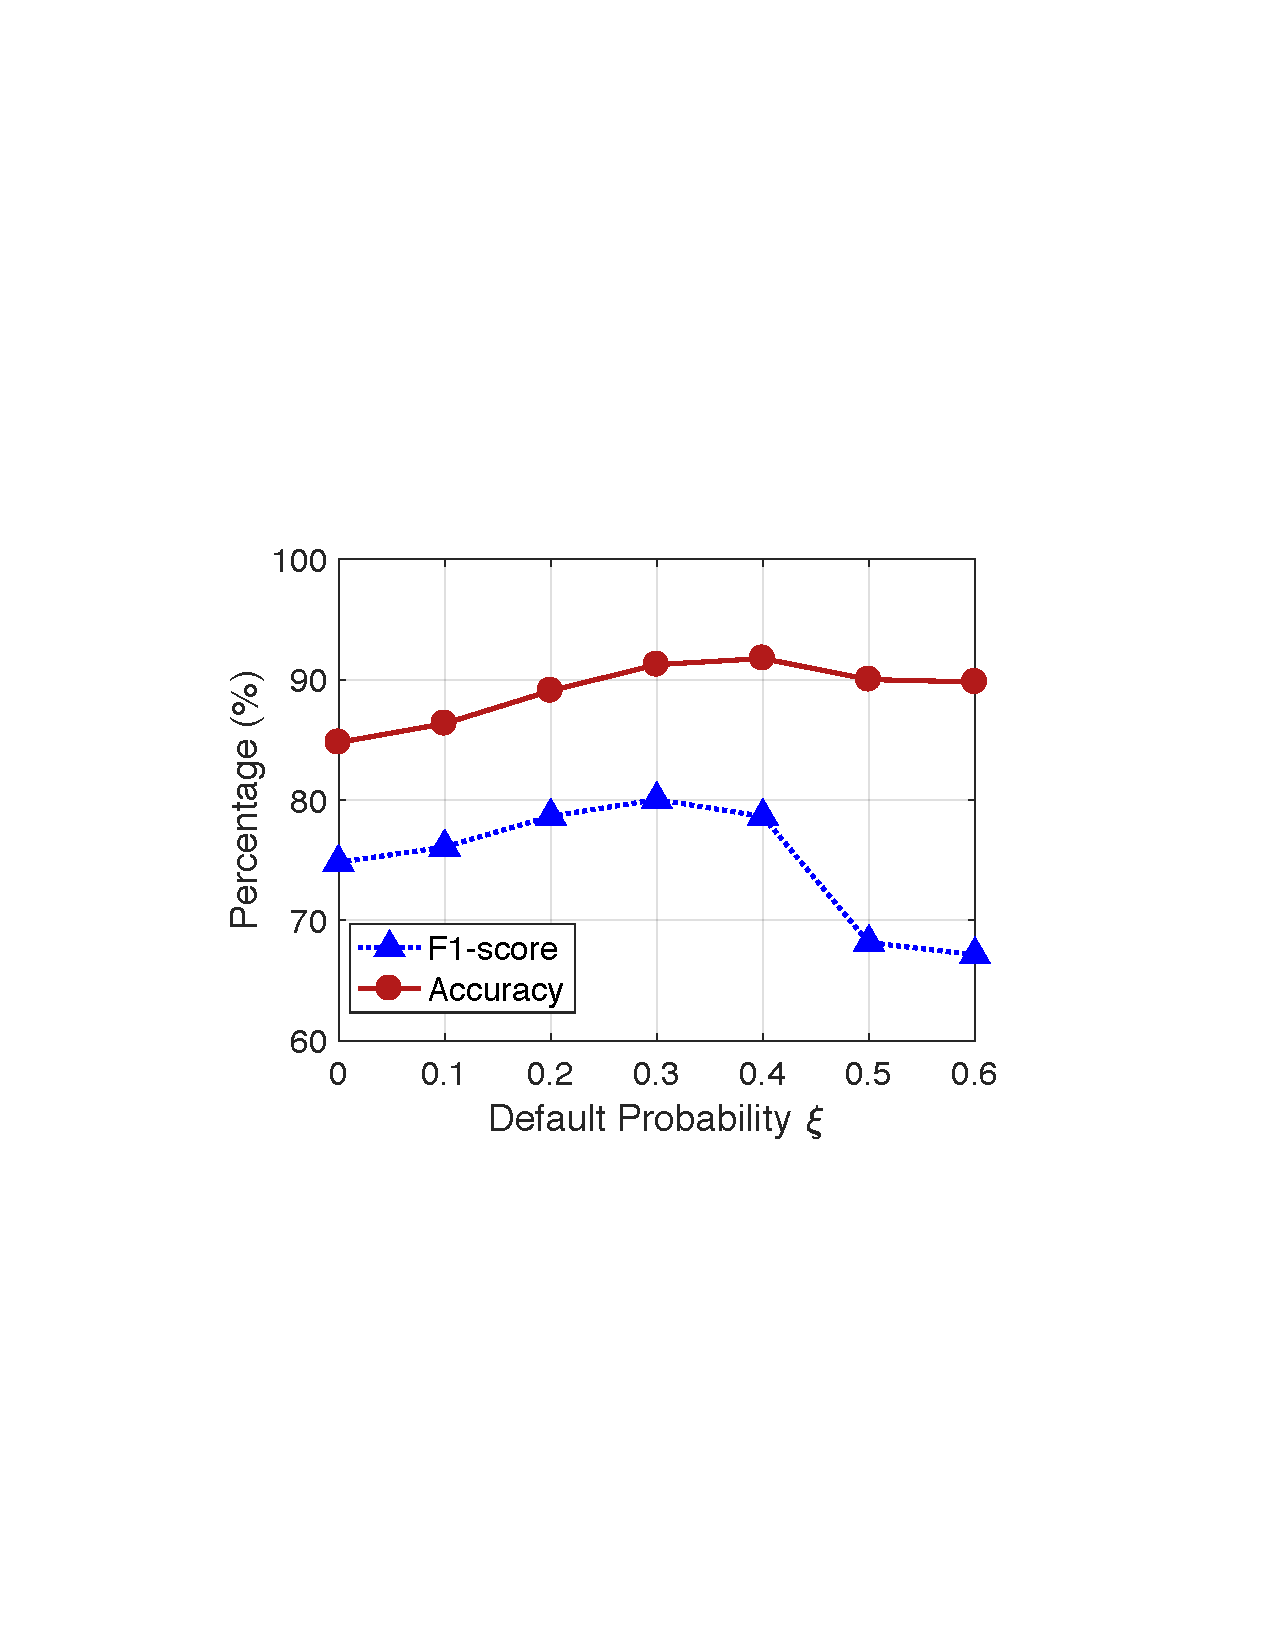
\includegraphics [width=0.235 \textwidth]{XiPercentage.pdf}
 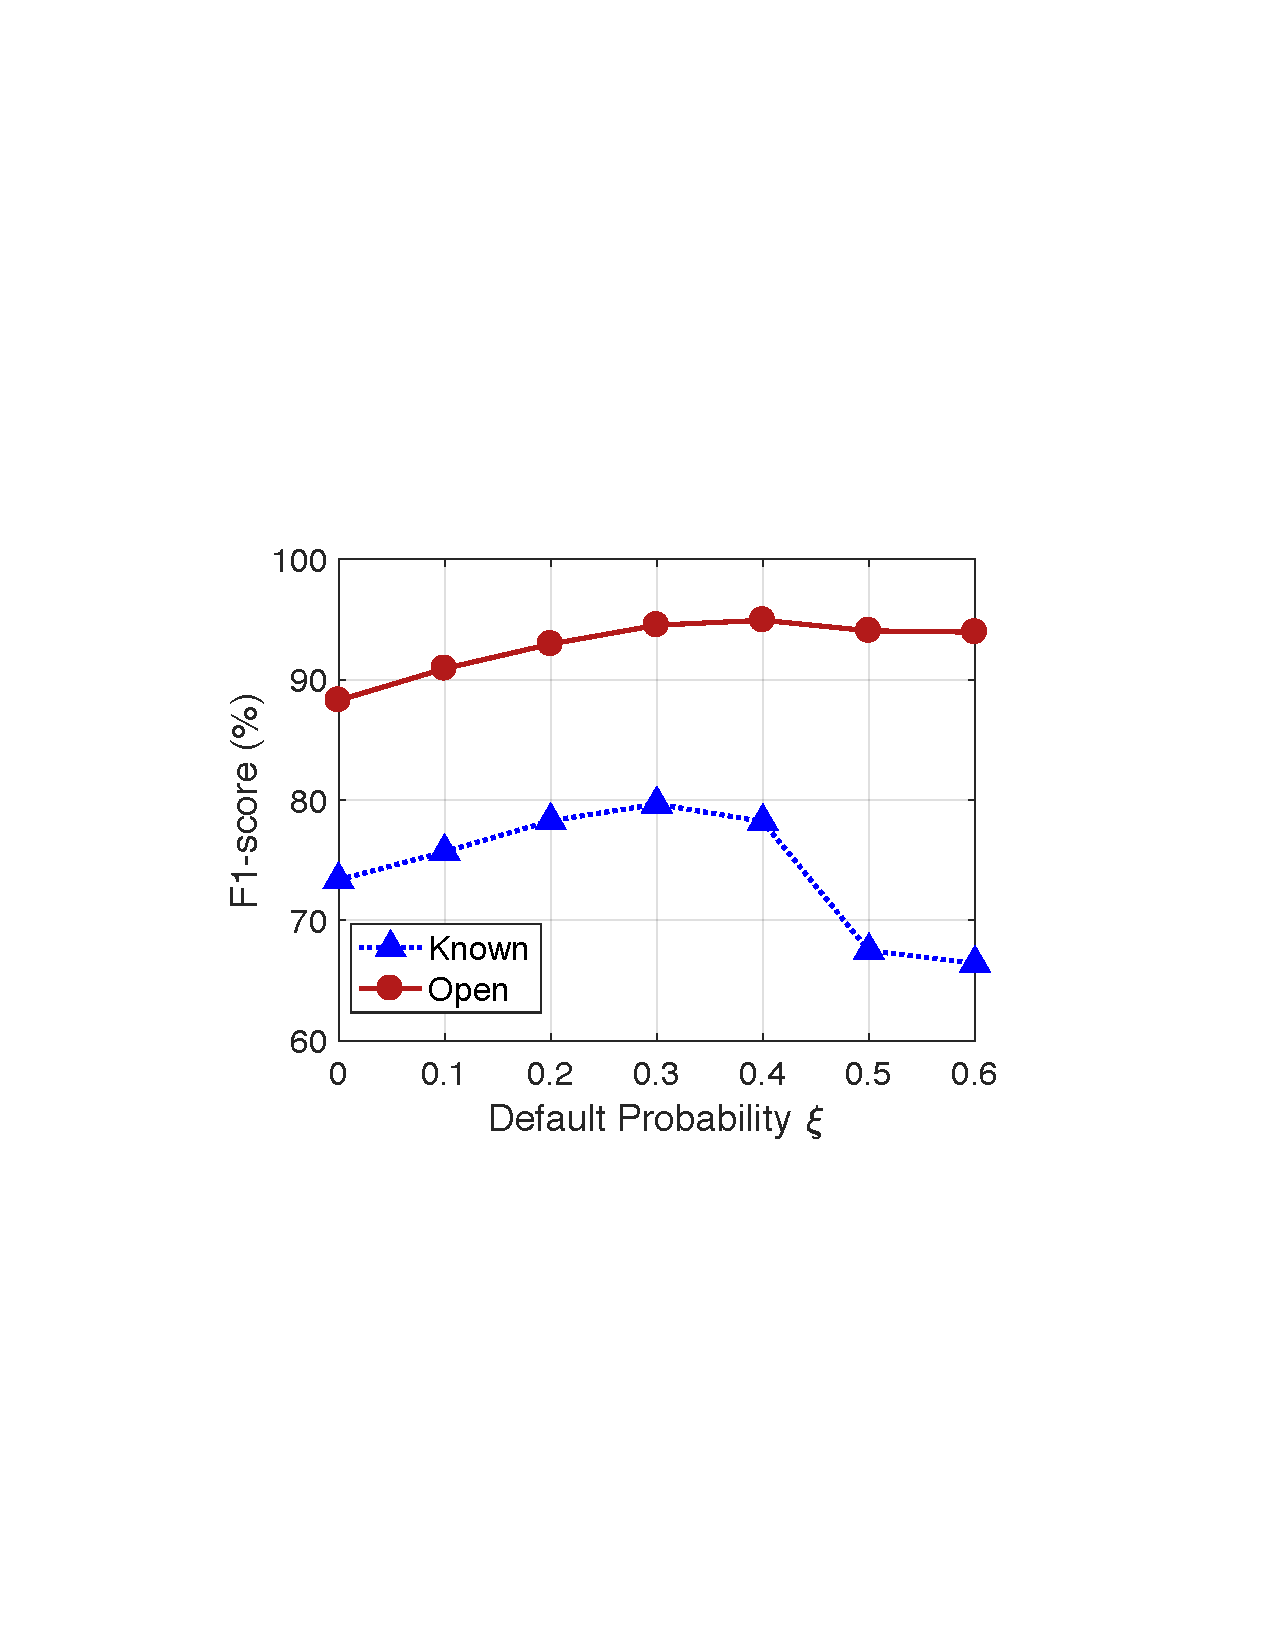
\includegraphics [width=0.235 \textwidth]{XiF1Score.pdf}
  }
  \subfigure[Effects of the tradeoff parameter $\mu$ in loss function.]{
         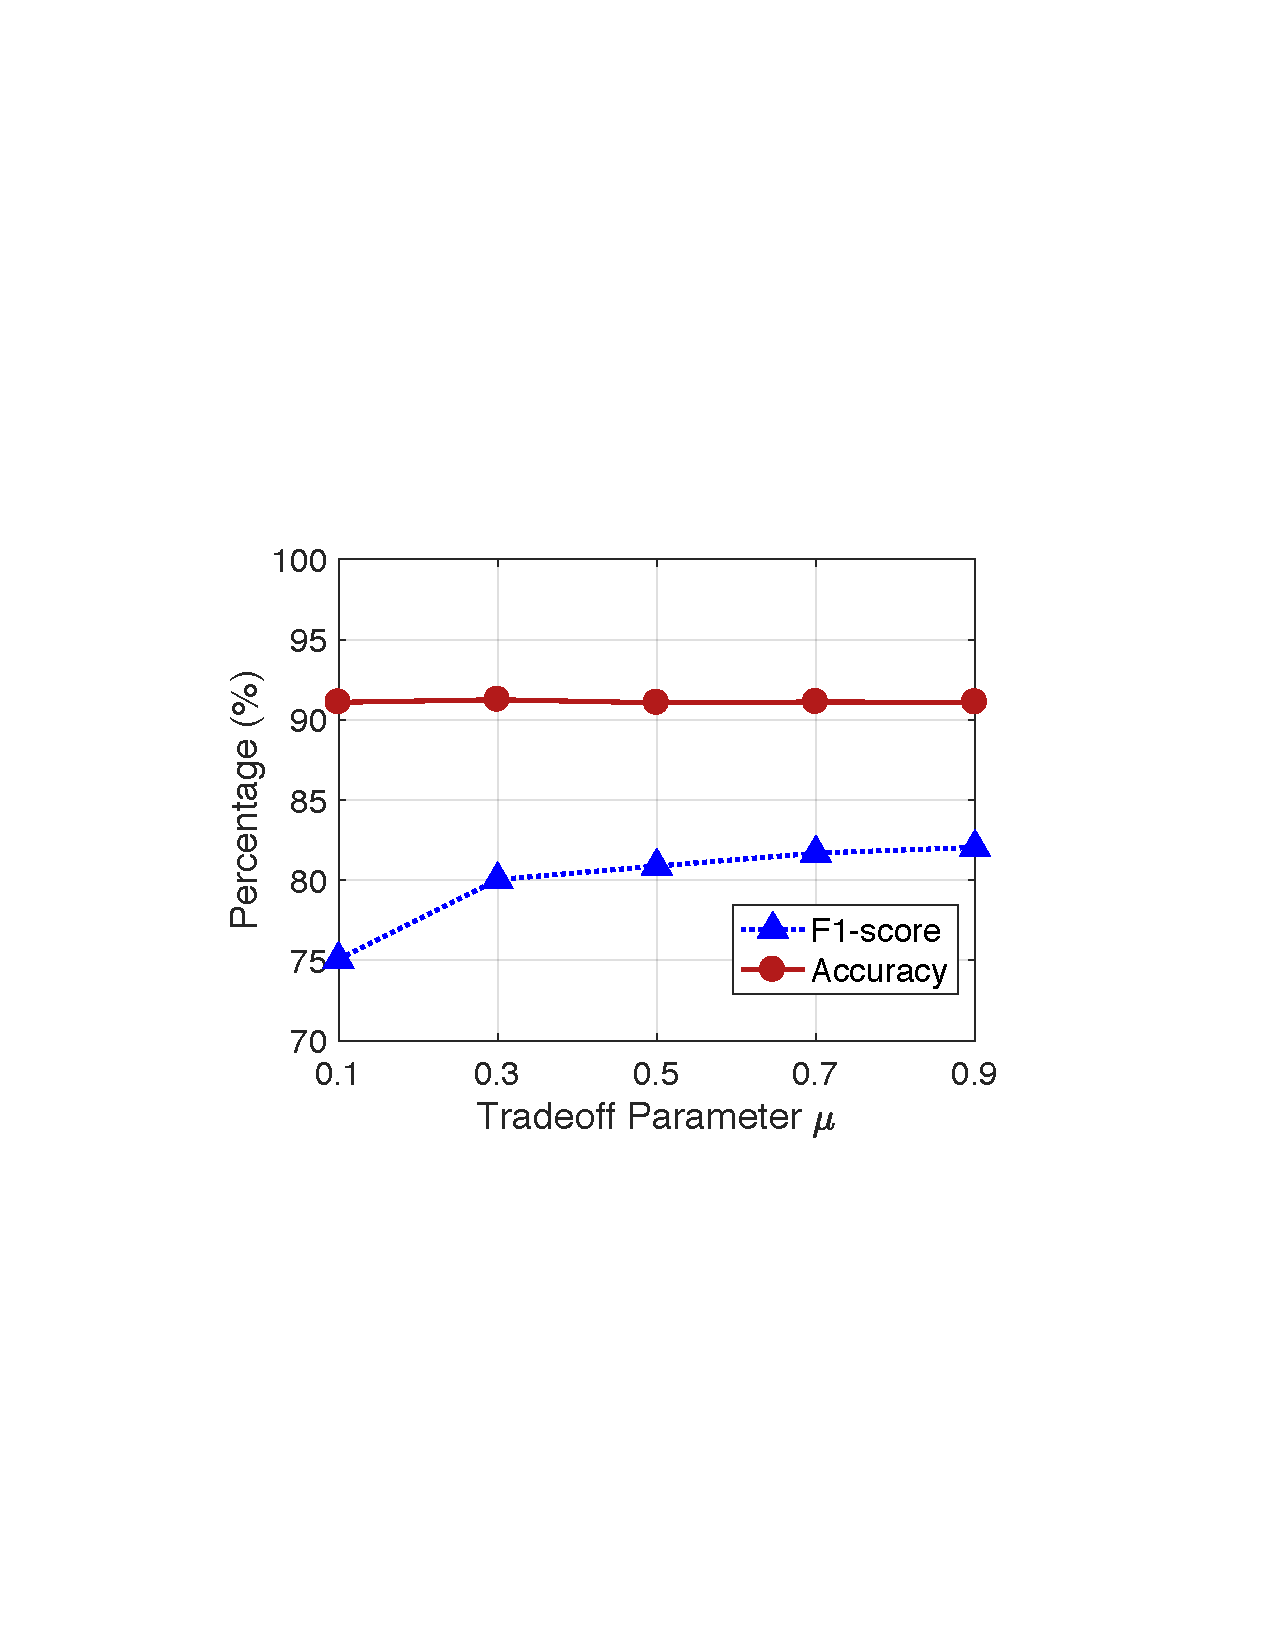
\includegraphics [width=0.235 \textwidth]{MuPercentage.pdf}
  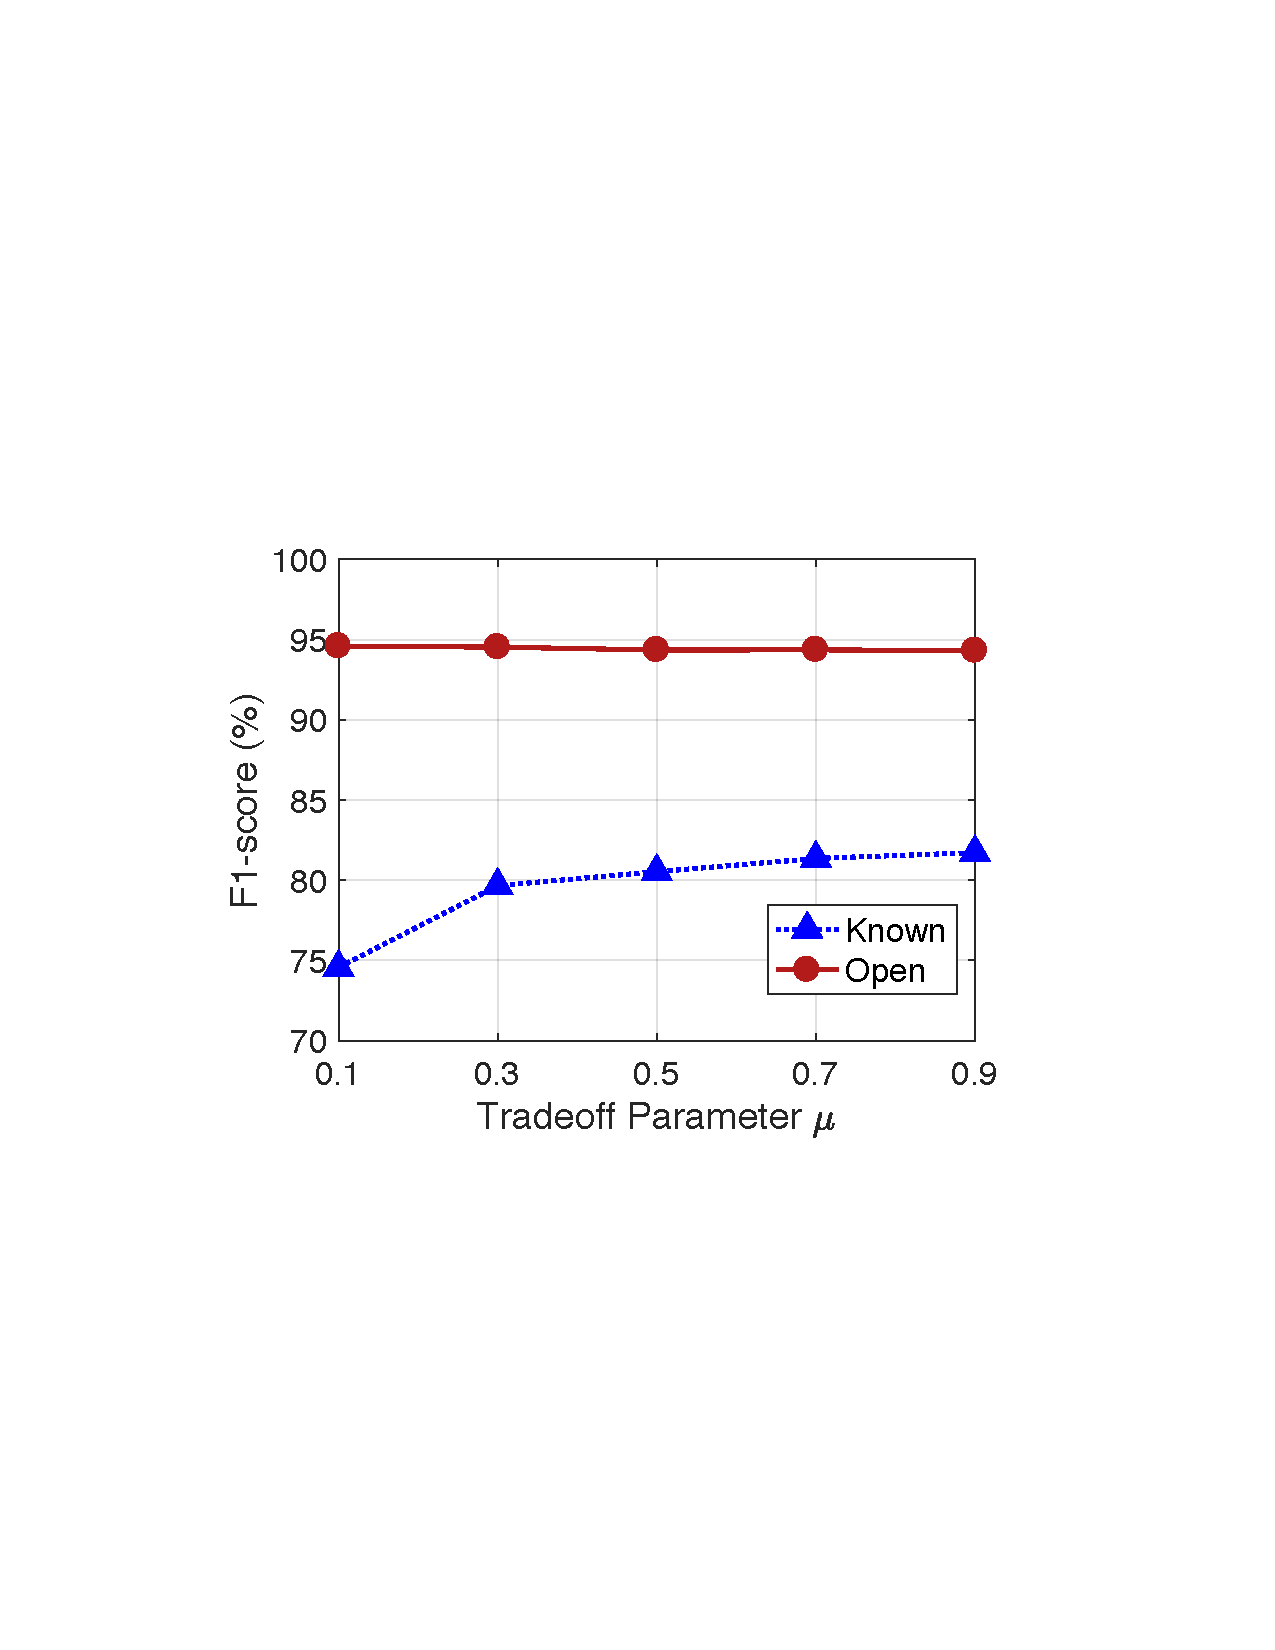
\includegraphics [width=0.235 \textwidth]{MuF1Score.pdf}
  }
  \caption{Effects of $\xi$ and $\mu$ on CLINC dataset with 25\% known classes. Left part is the effect of $\xi$ and the right part is the effect of $\mu$.} \label{hyper}
\end{figure*}


\subsection{Ablation Study}
In this section, we conduct experiments to explore the effects of pre-training, soft labeling, and manifold mixup on our model.
To conduct a comprehensive analysis, we report the performance on four metrics: accuracy, F1, weighted-F1, and Acc-KoK.
Among these metrics, weighted-F1 is mainly used to show the impact of class imbalance, and Acc-KoK is mainly used to analyze the impact of each component on the known intent classification under the closed-world setting.

First, as shown in Table \ref{tab:aba}, by observing the overall performance on accuracy, macro-F1, and weighted-F1, we can find that the performance drops after removing each of the three components (i.e., pre-training, SL, and MM) individually.
This indicates that all components contribute to the final performance.

Second, by observing the performance of removing pre-training, we can find that the accuracy drops by about 7\%, 8\%, and 7\% with three settings respectively.
This indicates that pre-training for known intents can learn better intent representation and is necessary for the training of SLMM.

Third, by observing the performance of removing soft labeling (implemented by setting $\xi = 0$), we can find that the accuracy of removing soft labeling drops by 6.47\%, 25.2\%, and 16.1\% with three settings respectively.
This shows that soft labeling is effective.
%And manifold mixup can improve model performance to a certain extent (e.g., w/o SL outperforms w/o SL\&MM by 65\%, 23.89\%, and 12.89\%  on accuracy with three settings).

Fourth, by observing the performance of removing manifold mixup (i.e., w/o MM), we can find that the accuracy and weighted-F1 consistently decreases, but the macro-F1 rises a little when the known intent ratio is 25\% and 50\%.
Such inconsistency trend of metrics is mainly caused by the class imbalance.
Since MM strategy only generate pseudo samples of open intents, MM makes the model more inclined to improve the performance on open intent class while degrading the performance on known intent classes.
Thus, when the ratio of open intents is large but the class weights are the same, the improvement on open intent class can not be effectively reflected by macro-F1.
From the perspective of accuracy and weighted-F1, we can find that MM can further improve the performance of our method upon the using of SL.
When the amount of data is more (i.e., 75\% known classes), macro F1-score over all classes drops.

Fifth, we can see that the model performs poorly after removing both soft labeling and manifold mixup.
This is because after removing soft labeling and manifold mixup, the model is only trained for known classes and cannot identify the open class.


\begin{figure*}
  \centering
        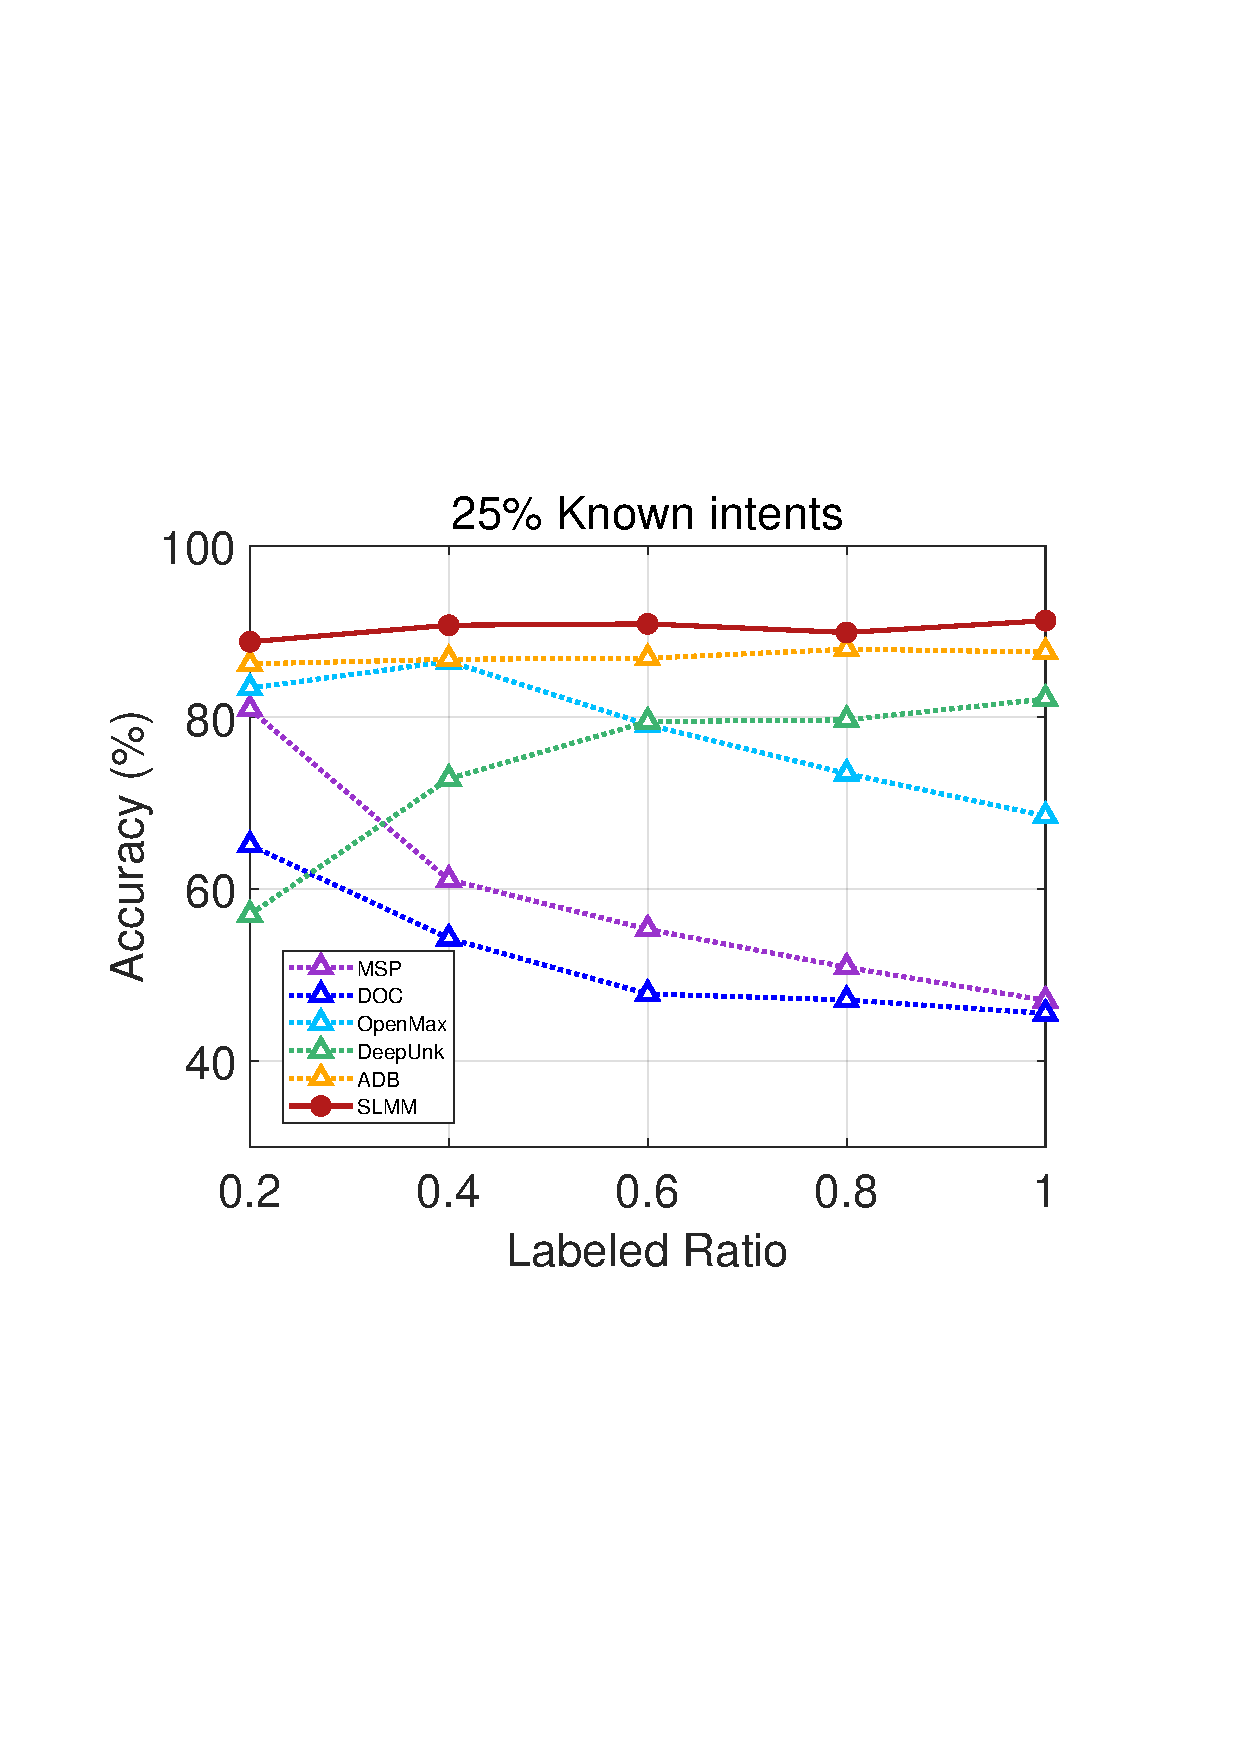
\includegraphics [width=0.3 \textwidth]{LabeledRatio25.pdf}
        \hspace{2mm}
 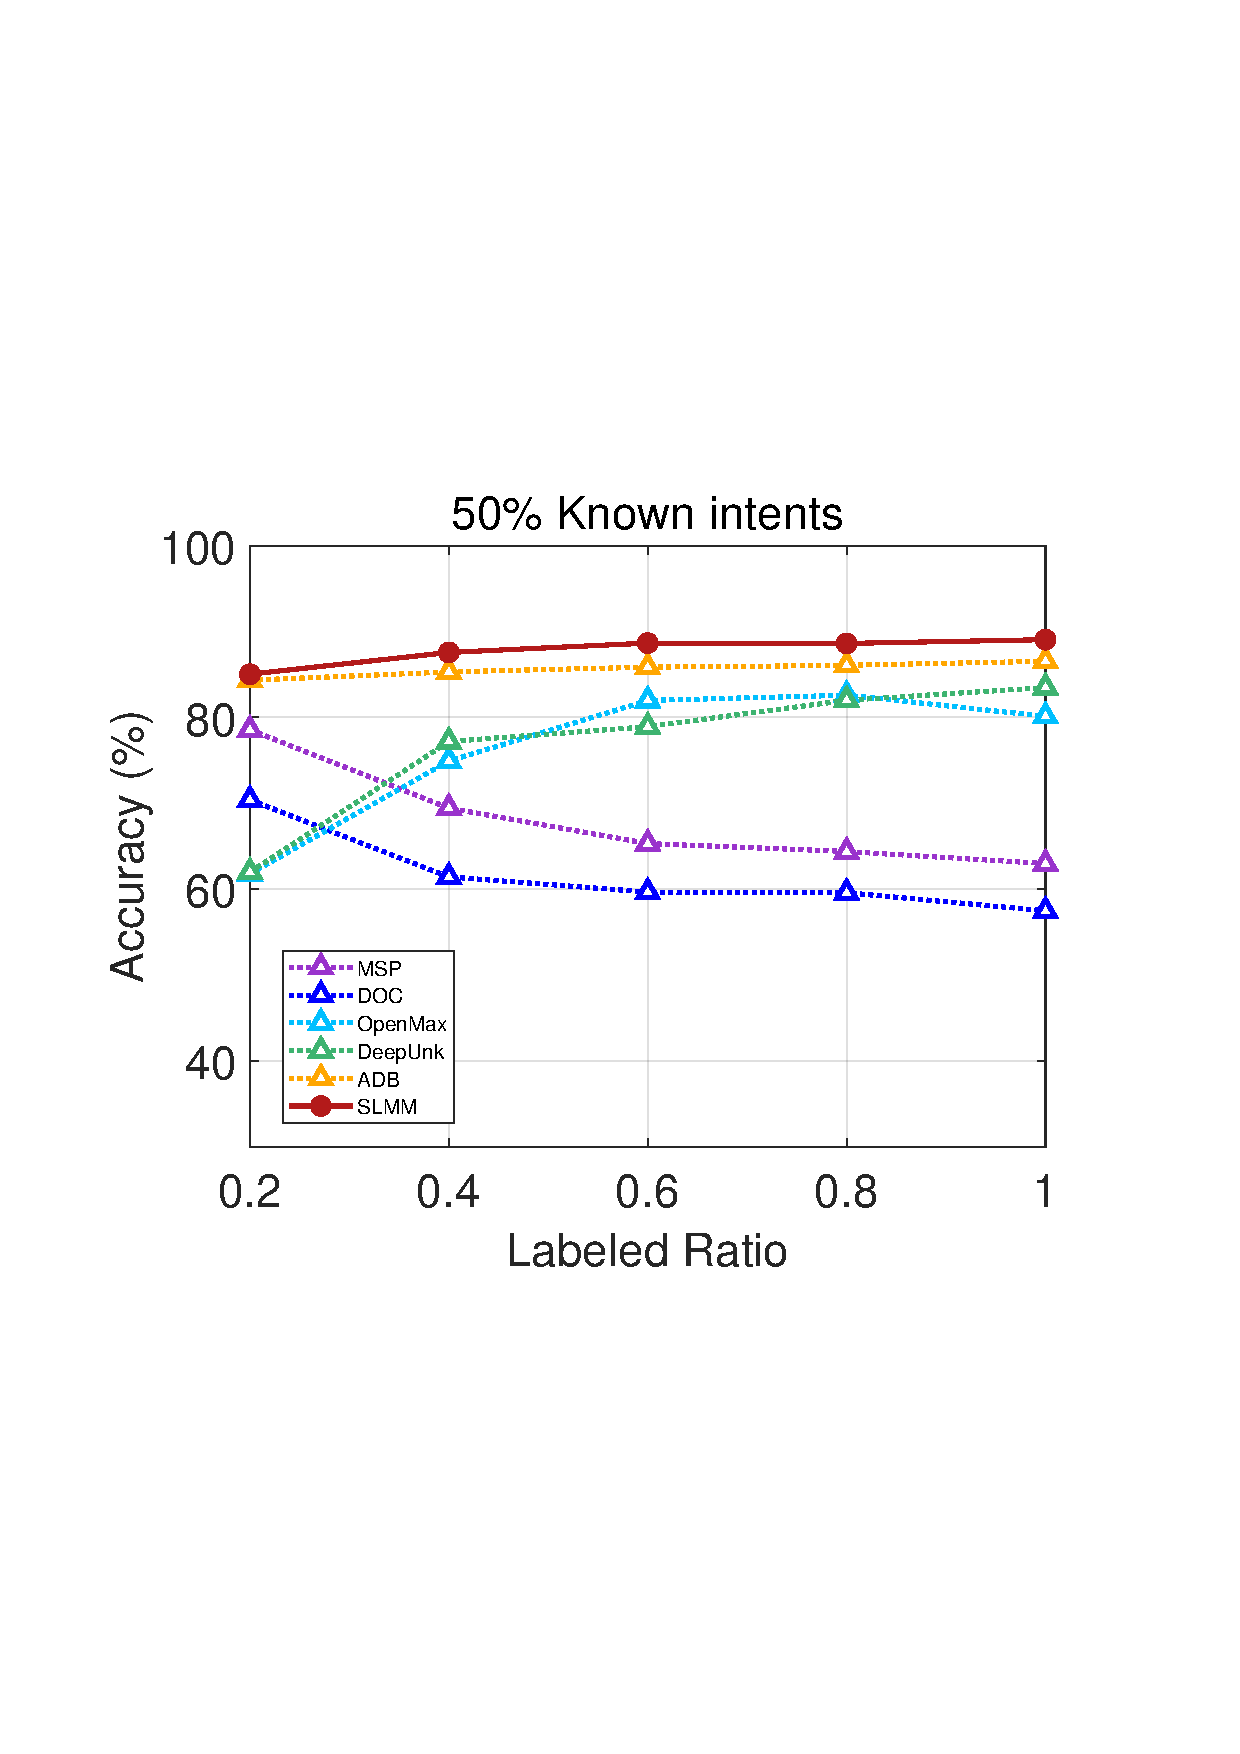
\includegraphics [width=0.3 \textwidth]{LabeledRatio50.pdf}
 \hspace{2mm}
 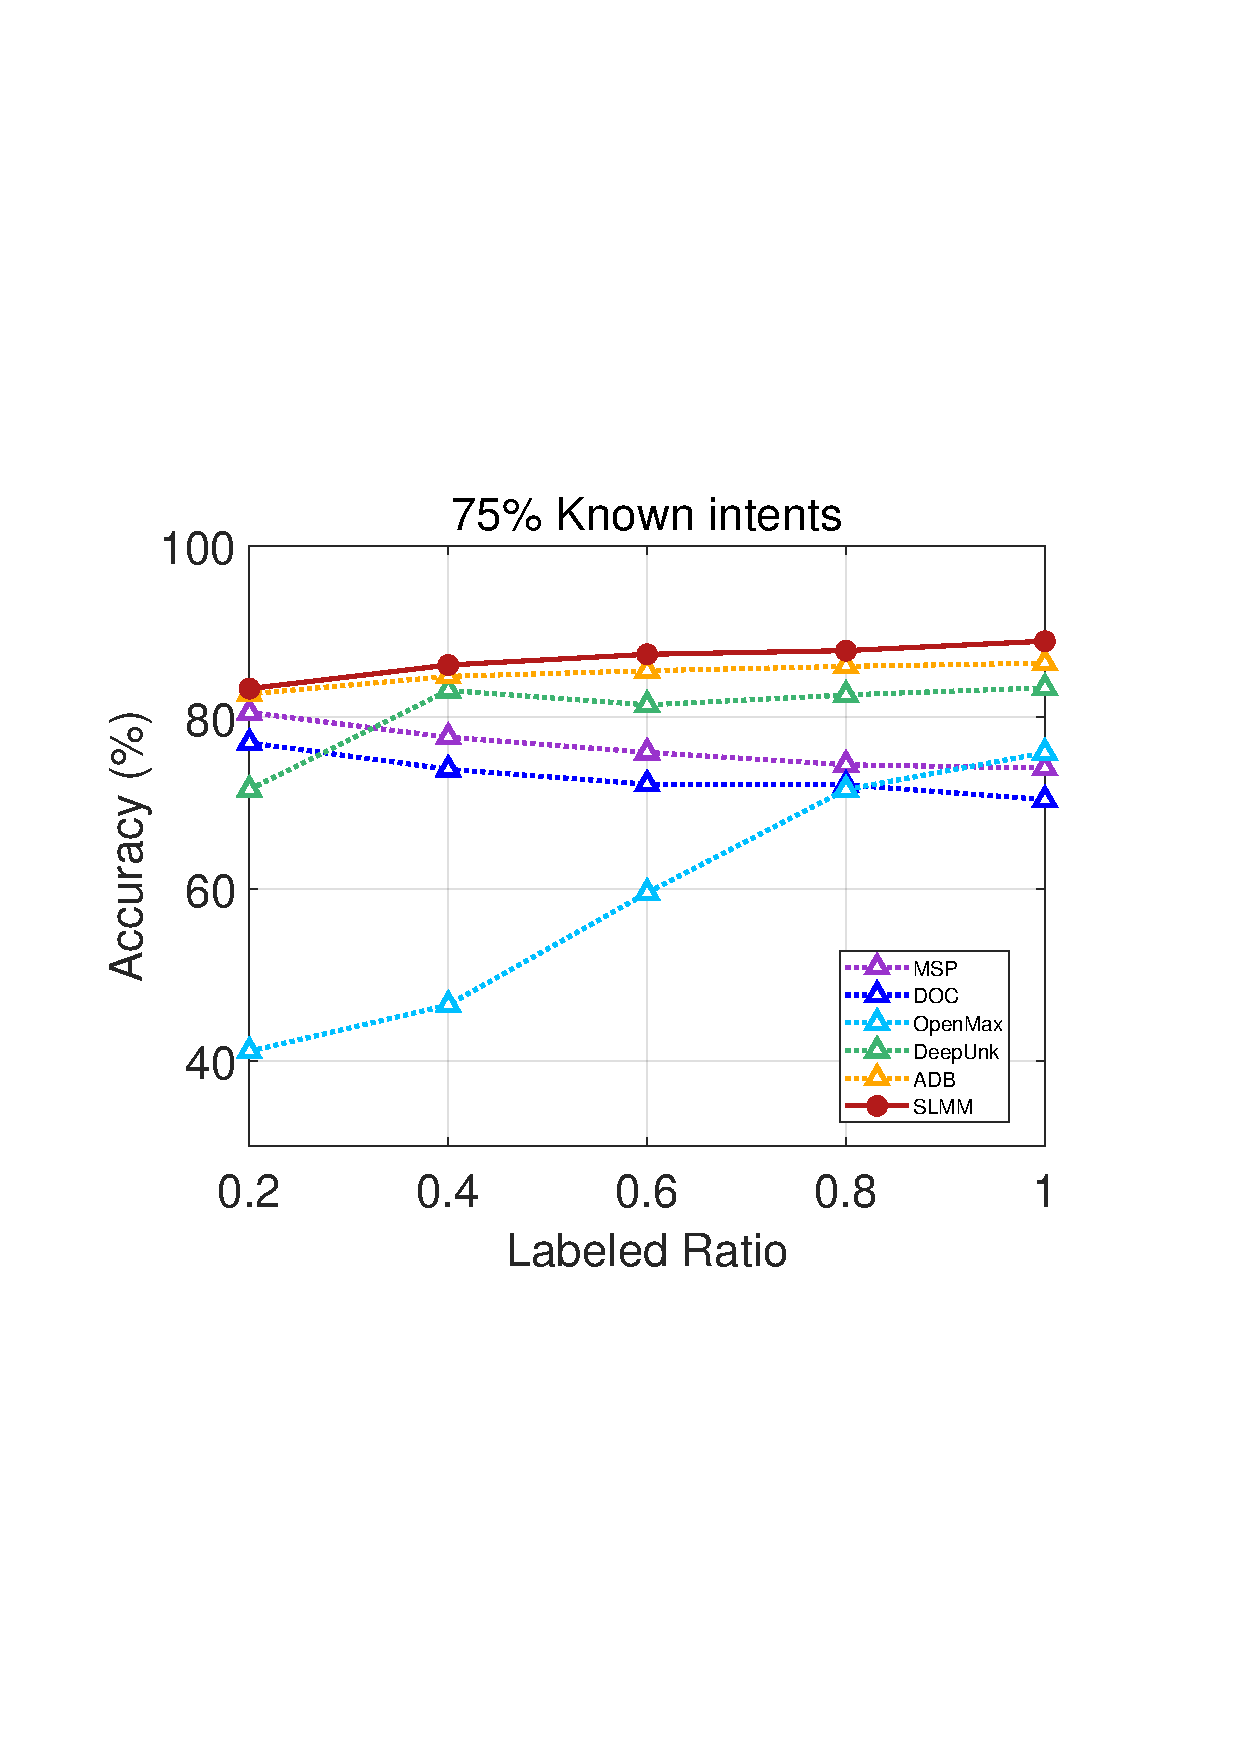
\includegraphics [width=0.3 \textwidth]{LabeledRatio75.pdf}
  \caption{Effects of the labeled ratio on CLINC dataset with different known class proportions (25\%, 50\%, 75\%).} \label{labeled}
\end{figure*}

Finally, we also list the accuracy of the known intent classifier on samples of known intents (i.e., Acc-KoK). 
We can find that using both SL and MM (i.e., SLMM) does not degrade the performance of the pre-trained konwn intent classification model (i.e., w/o SL\&MM), but using MM alone (i.e., w/o SL) degrades the performance of pre-trained model. 
This implies that SL is very important to maintain the performance of the pre-trained model on samples of known intents.
The reason may be that the soft labeling strategy plays a role similar to label smoothing, thus it can help to improve the generalization performance of the model.



\subsection{Model Analysis}

\subsubsection{Effect of Soft Labeling}
In this part, we explore the effect of $\xi$ on the performance of our method, which controls the default probability of open class in soft labeling.
We conduct experiment by varying $\xi$ from 0 to 0.6 step by 0.1 on CLINC dataset with 25\% known classes.
As shown in Figure \ref{hyper}(a), the overall performance increases first and then decreases with varied $\xi$.
This is because as $\xi$ increases, the model can effectively alleviate overconfident prediction problem and identify open class.
When $\xi$ is equal to 0.3, the performance (i.e., F1-score) is best.
Then the bigger $\xi$ has a negative effect on predicting known classes and the performance decreases.
This is because a large $\xi$ will make the model more inclined to predict samples as open class, thus the F1-score of known classes will drop significantly.

\begin{table} \setlength{\tabcolsep}{10pt}
\centering
\caption{Effect of $\alpha$ of Beta distribution in manifold mixup.}\label{alpha}
\begin{tabular}{ccccccc}
\toprule
{\bm \alpha}&\textbf{0.5}&\textbf{1}&\textbf{2}&\textbf{4}\\
\midrule
\textbf{Accuracy} &81.50&90.22&91.25&\bf{91.85} \\
\textbf{F1}&15.08&69.78&\bf{80.04}& 79.79\\
\bottomrule
\end{tabular}
\end{table}


% final version : no blue
\begin{table} \setlength{\tabcolsep}{15pt}
\centering
\caption{Effect of interpolation position $n$ in manifold mixup.} \label{n}
\begin{tabular}{ccccccc}
\toprule
\textbf{n}&\textbf{9}&\textbf{10}&\textbf{11}\\
\midrule
\textbf{Accuracy} &87.03&86.85&\bf{91.25} \\
\textbf{F1}&75.30&75.18&\bf{80.04}\\
\bottomrule
\end{tabular}
\end{table}

\iffalse
\begin{table} \setlength{\tabcolsep}{15pt}
\centering
\caption{\textcolor{blue}{Effect of interpolation position $n$ in manifold mixup.}} \label{n}
\begin{tabular}{ccccccc}
\toprule
\textcolor{blue}{\textbf{n}}&\textcolor{blue}{\textbf{9}}&\textcolor{blue}{\textbf{10}}&\textcolor{blue}{\textbf{11}}\\
\midrule
\textcolor{blue}{\textbf{Accuracy}} &\textcolor{blue}{87.03}&\textcolor{blue}{86.85}&\textcolor{blue}{\bf{91.25}} \\
\textcolor{blue}{\textbf{F1}}&\textcolor{blue}{75.30}&\textcolor{blue}{75.18}&\textcolor{blue}{\bf{80.04}}\\
\bottomrule
\end{tabular}
\end{table}
\fi



\subsubsection{Effect of Manifold Mixup}
In this part, we explore the effect of $\alpha$ and $n$ on the performance of our method, which are hyperparameters of Beta distribution and interpolation position in manifold mixup.
We conduct experiment by varying $\alpha$ (i.e., 0.5, 1, 2, and 4) and $n$ (i.e., 9, 10, and 11) on CLINC dataset with 25\% known classes.
First, we explore the effect of $\alpha$.
When $\alpha$ equals to 0.5, the sampled $\lambda$ from Beta distribution is near 0 or 1.
When $\alpha$ equals to 1, the sampled $\lambda$ is uniform.
When $\alpha$ equals to 2 or 4, the sampled $\lambda$ is close to 0.5.
As shown in Table \ref{alpha}, $\alpha$ has a significant impact on performance.
When $\alpha$ is equal to 0.5 or 1, the model does not perform well.
This is because the quality of the generated samples is poor, and their representation is close to samples of known classes (i.e., high-confidence areas).
This makes the model confused about distinguishing between samples of known classes and open class. 
When $\alpha$ is equal to 2 or 4, the model performs well.
This is due to the generated samples are in the low-confidence areas, and these samples can help model to learn a better decision boundary.
When $\alpha$ is equal to 2 or 4, the overall performance does not change much.
So we set $\alpha$ = 2 by default.
Second, we explore the effect of $n$.
From Table~\ref{n}, we can find that when $n$ equals to 11, model achieves the best performance.
The performance of setting smaller $n$ is worse than that of setting $n=11$.
This may be because we fix all the parameters of BERT but the last layer and previous fixed transformer layers cannot effectively adapt to the change of representation mode brought by manifold mixup.

\begin{figure}
\centering
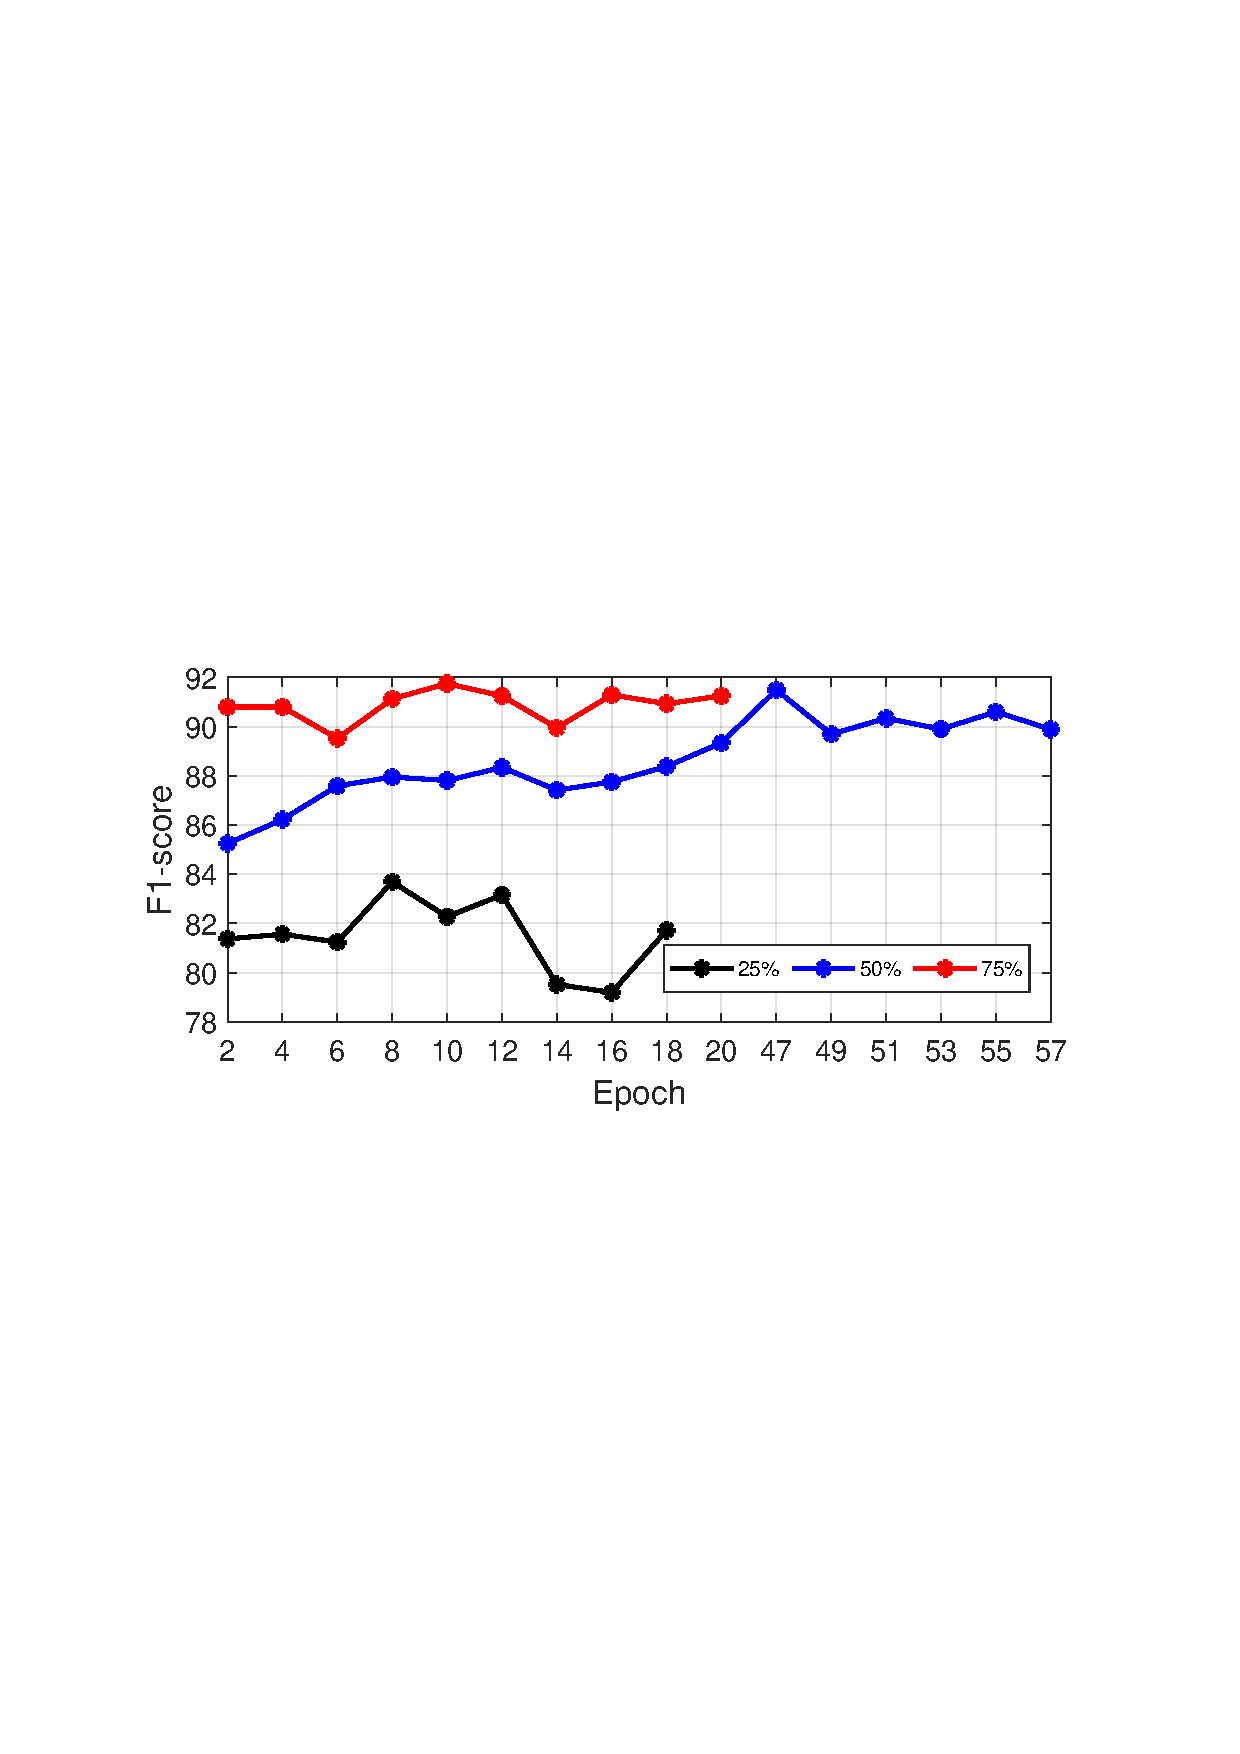
\includegraphics[width=0.8\columnwidth]{iteration.pdf}
\caption{The performance of our method on the validation set of CLINC dataset with the increase of training epoch.} \label{learning_process}
\end{figure}

\subsubsection{Effect of Tradeoff Parameter}
In this part, we explore the effect of the tradeoff parameter $\mu$ on the performance of our method.
We conduct experiment by varying $\mu$ from 0.1 to 0.9 step by 0.2 on CLINC dataset with 25\% known classes.
The results are shown in Figure \ref{hyper}(b).
We can observe that SLMM achieves the relatively stable performance on accuracy with varied $\mu$, which indicates the robustness of our method.
When $\mu = 0.3$, we can get the best accuracy.
As $\mu$ increases, macro F1-score over open class decreases slightly and macro F1-score over all classes and known classes rises.
This is because as $\mu$ increases, model will pay less attention to pseudo samples generated through manifold mixup and is more inclined to predict samples as known intent classes.
And macro F1-score over all classes is closer to macro F1-score over known classes.
Therefore, macro F1-score over all classes and known classes have an upward trend, and macro F1-score over open class has a downward trend.


\subsubsection{Effect of Labeled Data}
In this part, we explore the effect of labeled data by varying the labeled ratio in the range of 0.2, 0.4, 0.6, 0.8, and 1.0 on CLINC dataset with 25\%, 50\%, and 75\% known intent classes.
First, we can see that our model achieves the best performance on all settings as shown in Figure \ref{labeled}.
This shows the effectiveness of our method.
And the advantage of our method is more obvious, when the amount of labeled data is small with 25\% known intents.
%This shows that even when the amount of labeled data is very limited, our method can effectively distinguish the known classes between open class.
Second, we can see that the performance of our model is stable, and the statistic-based methods (i.e., MSP and DOC) only work well with less labeled data and perform poorly as the ratio of labeled data increases.
This is because these methods tend to be biased towards the known intent classes as the number of labeled data increases.
Some deep learning methods (i.e., OpenMax and DeepUnk) perform poorly with less labeled data.
This is because the centroids and representations learned by their method are biased with less labeled data.
Both our method and ADB achieve stable performance, but our method achieves a better performance than ADB.


\subsubsection{Effect of Training Epoch}
We further explore how the performance of our method varies on validation set with the increase of training epoch.
As shown in Figure~\ref{learning_process}, three lines are drawn corresponding to three settings of known intent ratio (i.e., 25\%, 50\%, and 75\%) on the CLINC dataset.
To avoid endless training, we set the maximum training epoch as 100, but early stop the training if the best performance on validation set is not updated for 10 consecutive epochs.
As shown, the lines of 25\%, 50\%, and 75\% complete the training process with early stopping at the 18th, 57th, and 20th epoch respectively.
The best performance of our method on validation set is thus achieved at the 8th, 47th, and 10th epoch respectively for the three settings.
The fact that so many epochs are needed to retrain the model implies that the SLMM phase made a large adjustment to the representation space of the pre-training step.


\begin{figure}[t]
\centering
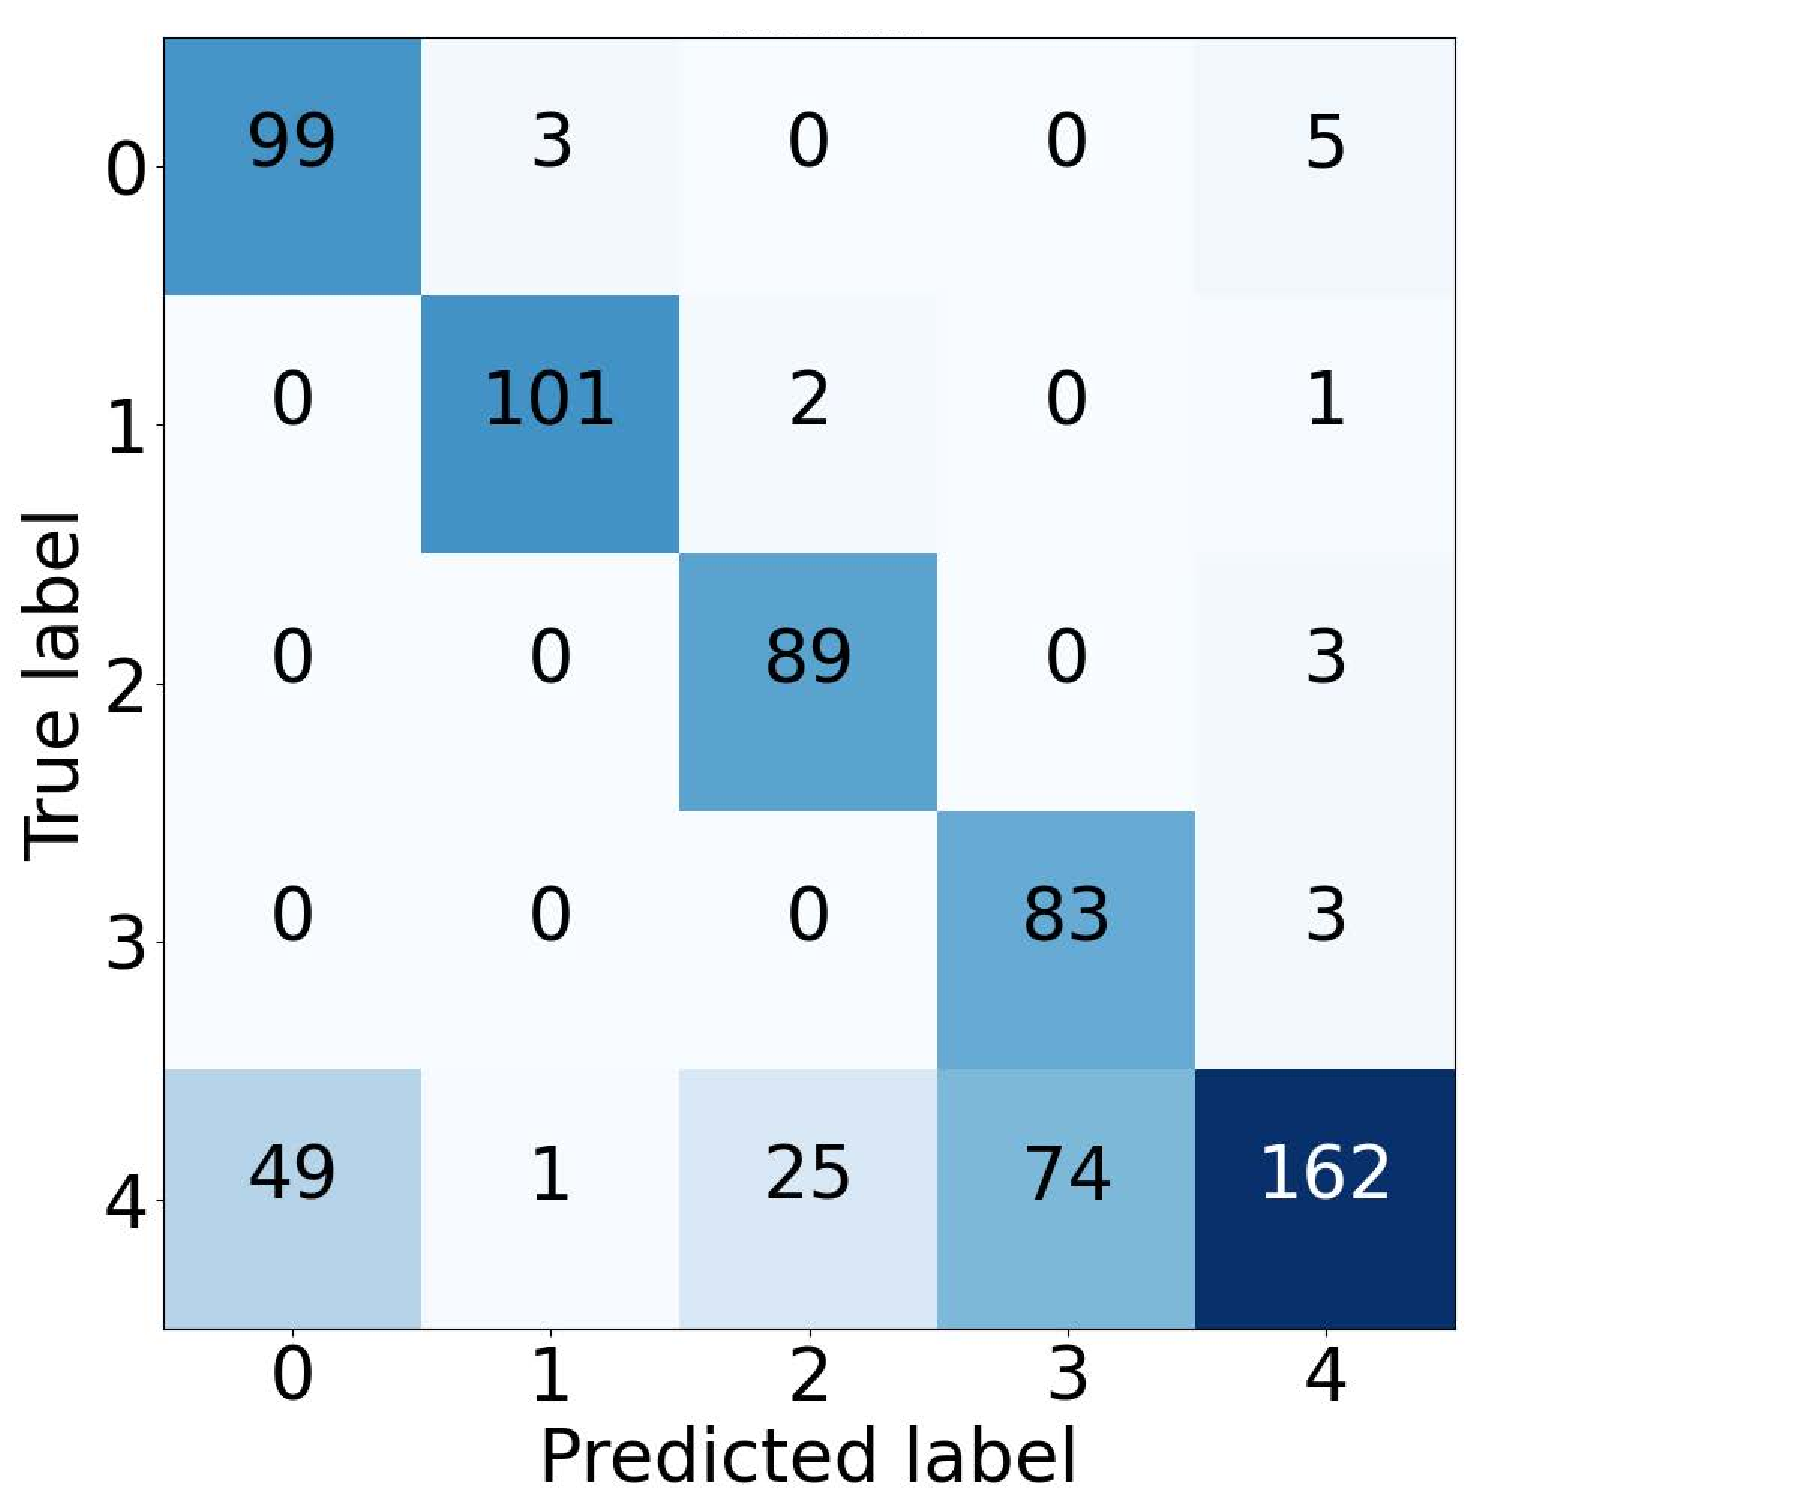
\includegraphics[width=0.5\columnwidth]{matrix.pdf}
\caption{Confusion matrix of our model on SNIPS dataset with 50\% known classes. Class 4 denotes the open class.}\label{cm}
\end{figure}

\begin{table}\scriptsize\setlength{\tabcolsep}{1pt}
\centering
\caption{Two examples for error analysis.} \label{case_study}
\begin{tabular}{l|c|c}
\toprule
\textbf{Utterance} & \textbf{Ground-Truth Intent} &\textbf{Predicted Intent}\\
\midrule
Add this song to blues roots. & \tabincell{c}{Add To Play List \\ \emph{\textbf{Open intents}}} & \tabincell{c}{Play Music \\ \emph{\textbf{Known intents}}}\\
\midrule
Find a movie called living in america. & \tabincell{c}{Search Creative Work \\ \emph{\textbf{Open intents}}} &  \tabincell{c}{Search Screening Event \\ \emph{\textbf{Known intents}}}\\
\bottomrule
\end{tabular}
\end{table}


\subsection{Error Analysis}


\begin{figure*}
  \centering
    \subfigure[50\% known classes on SNIPS.]{
         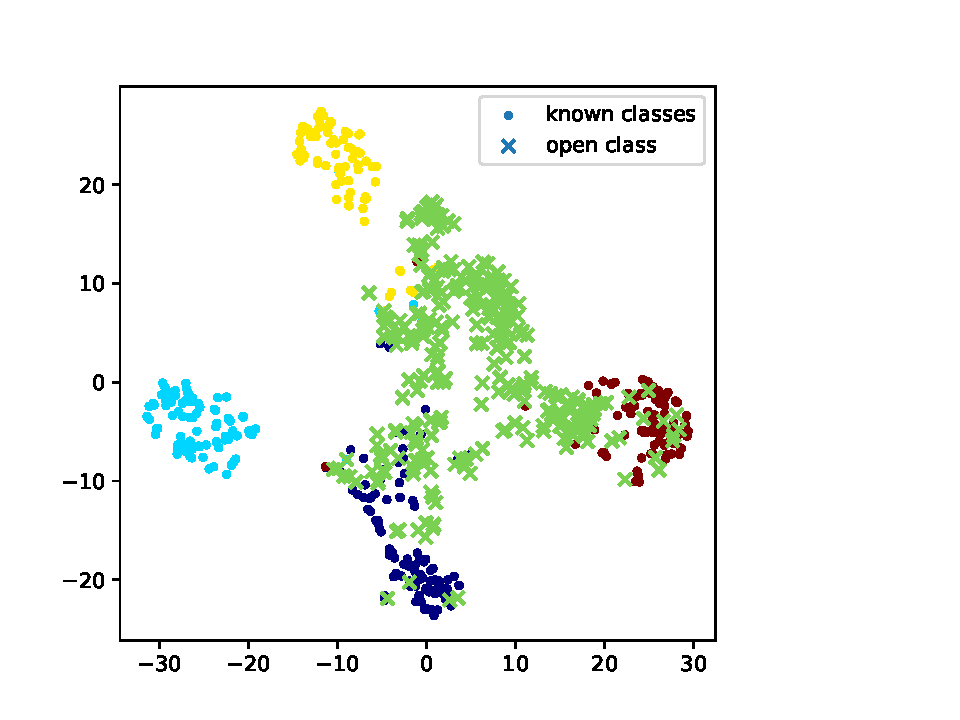
\includegraphics [width=0.27 \textwidth]{T-SNE.pdf}}\hspace{8mm}
  \subfigure[75\% known classes on CLINC.]{
        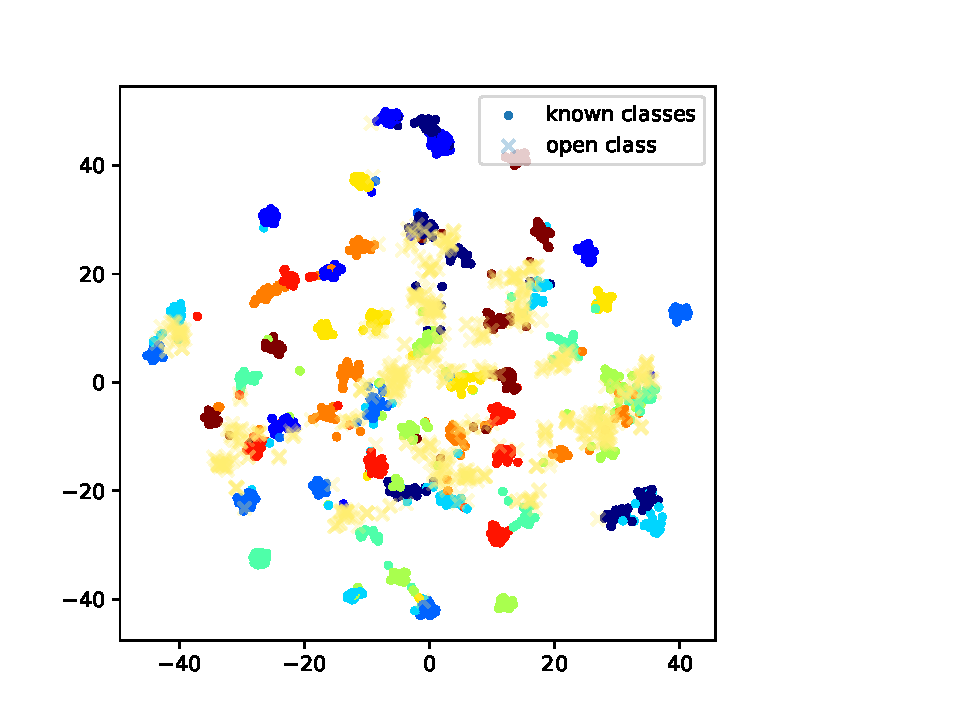
\includegraphics [width=0.27 \textwidth]{t-sne-banking.pdf}
        }\hspace{8mm}
        \subfigure[75\% known classes on OOS.]{
 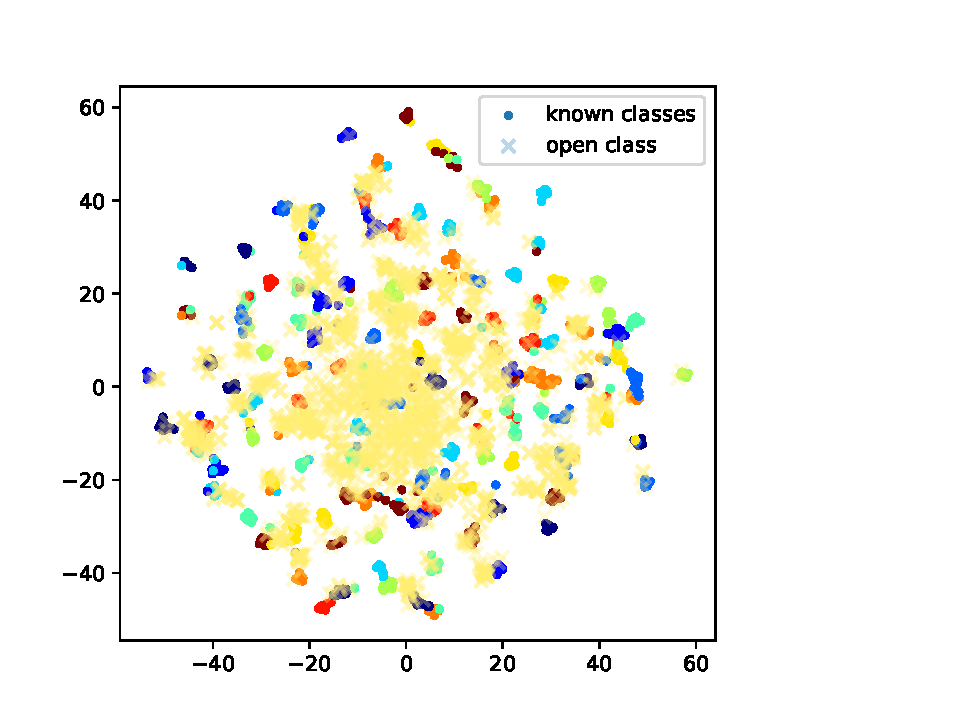
\includegraphics [width=0.27 \textwidth]{t-sne-oos.pdf}
  }
  \caption{Visualization of the learned embeddings from test set on three datasets.} \label{t-sne}
\end{figure*}

In this section, we perform error analysis on our model and report the confusion matrix under 50\% known classes on SNIPS dataset in Figure~\ref{cm}.
We can see that the off-diagonal elements can be divided into two types of errors: open class related error and known classes error.
First, we can find that open class related error occupies a large proportion of errors and many samples of open class have not been recognized.
For example, 49 samples of open class are predicted as label 0 and 74 samples of open class are predicted as label 3. 
There is also a small part of samples of known classes that are recognized as open class.
Second, there are five samples belonging to known classes error.
For example, 3 samples of class 0 are predicted as label 1 and 2 samples of class 1 are predicted as label 2.
This shows that our model can distinguish the known classes well, and the identification of the unknown classes is still the main challenge at present.
It is worth noting that it is hard to distinguish between label 3 and label 4.
By further observing the errors produced by the model on the SNIPS dataset, we found that some open intents are very similar with some known intents.
This makes it easy for these open intents to be classified as known intents, and thus producing errors.
For example, as shown in Table~\ref{case_study}, in the first case, it is hard to distinguish between the known intent `Play Music’ and the open intent `Add To Play list’.
This maybe because the utterances of these two intent classes are similar on vocabulary and semantics, and thus the features learned for these utterances are also hard to distinguish.
The second case shows a similar phenomenon.

\iffalse
\begin{figure}[t]
\centering
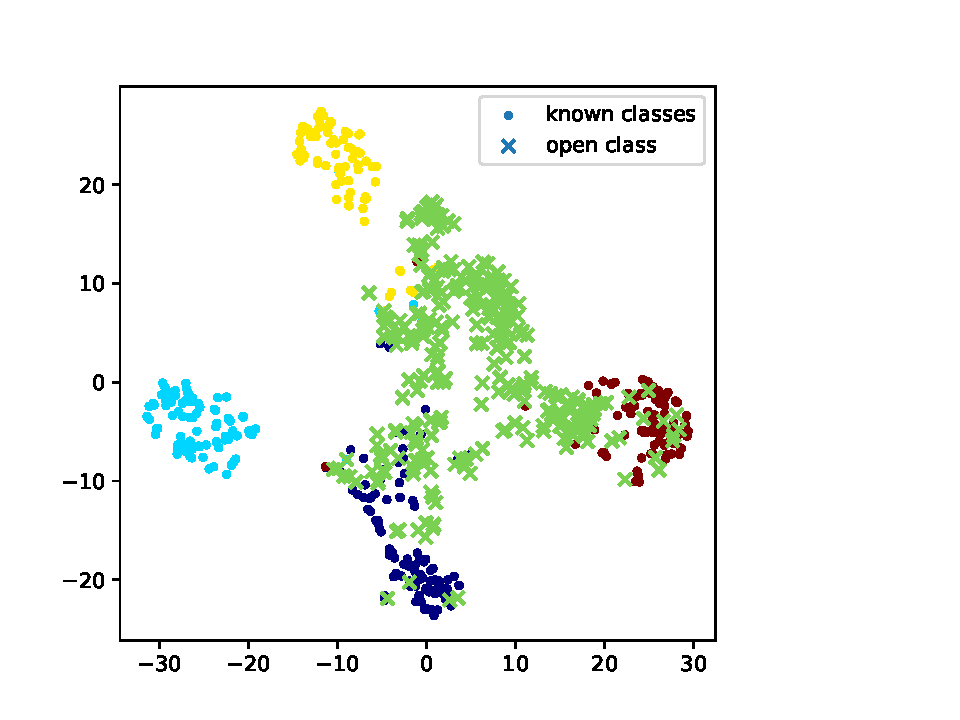
\includegraphics[width=0.7\columnwidth]{T-SNE.pdf}
\caption{t-SNE \cite{van2008visualizing} visualization of the learned embeddings from test set on SNIPS dataset with 50\% known classes.}\label{t-sne}
\end{figure}
\fi


\subsection{Visualization}

In this section, we visualize the embeddings of samples in test set by t-SNE \cite{van2008visualizing}.
As shown in Figure \ref{t-sne}, we plot three subfigures corresponding to three datasets: SNIPS, BANKING, and OOS, where the ratio of known classes are 50\%, 75\%, and 75\% respectively.
Among these subfigures, the samples of open class and known classes are represented as forks and dots, respectively.
From these subfigures, we can see that the learned embeddings can be separated well.
This shows that our method is effective.
In addition, we can also find that the samples of open class are mostly placed near known classes or between two different known classes.
This is consistent with our intuition of soft labeling and manifold mixup, and further shows the effective of our proposed two strategies.
Then this figure suggests, in agreement with results of Figure \ref{cm}, different known classes are better separated, and the main challenge is to identify open class.
It is worth noting that the difficulty of distinguishing between different known classes and open classes is different.


\section{Conclusion}
In this paper, we propose a deep open intent classification model based on soft labeling and manifold mixup.
Specifically, soft labeling gives each sample a probability of being predicted as an open intent, and manifold mixup generates open intent samples via interpolating between the hidden representation of two different known intent samples.
Through these two strategies, our model can directly perform (K+1)-class classification without outlier detection algorithms. 
We conduct extensive experiments on the benchmark datasets.
The experimental results demonstrate the effectiveness of our proposed method.




% An example of a floating figure using the graphicx package.
% Note that \label must occur AFTER (or within) \caption.
% For figures, \caption should occur after the \includegraphics.
% Note that IEEEtran v1.7 and later has special internal code that
% is designed to preserve the operation of \label within \caption
% even when the captionsoff option is in effect. However, because
% of issues like this, it may be the safest practice to put all your
% \label just after \caption rather than within \caption{}.
%
% Reminder: the "draftcls" or "draftclsnofoot", not "draft", class
% option should be used if it is desired that the figures are to be
% displayed while in draft mode.
%
%\begin{figure}[!t]
%\centering
%\includegraphics[width=2.5in]{myfigure}
% where an .eps filename suffix will be assumed under latex, 
% and a .pdf suffix will be assumed for pdflatex; or what has been declared
% via \DeclareGraphicsExtensions.
%\caption{Simulation results for the network.}
%\label{fig_sim}
%\end{figure}

% Note that the IEEE typically puts floats only at the top, even when this
% results in a large percentage of a column being occupied by floats.


% An example of a double column floating figure using two subfigures.
% (The subfig.sty package must be loaded for this to work.)
% The subfigure \label commands are set within each subfloat command,
% and the \label for the overall figure must come after \caption.
% \hfil is used as a separator to get equal spacing.
% Watch out that the combined width of all the subfigures on a 
% line do not exceed the text width or a line break will occur.
%
%\begin{figure*}[!t]
%\centering
%\subfloat[Case I]{\includegraphics[width=2.5in]{box}%
%\label{fig_first_case}}
%\hfil
%\subfloat[Case II]{\includegraphics[width=2.5in]{box}%
%\label{fig_second_case}}
%\caption{Simulation results for the network.}
%\label{fig_sim}
%\end{figure*}
%
% Note that often IEEE papers with subfigures do not employ subfigure
% captions (using the optional argument to \subfloat[]), but instead will
% reference/describe all of them (a), (b), etc., within the main caption.
% Be aware that for subfig.sty to generate the (a), (b), etc., subfigure
% labels, the optional argument to \subfloat must be present. If a
% subcaption is not desired, just leave its contents blank,
% e.g., \subfloat[].


% An example of a floating table. Note that, for IEEE style tables, the
% \caption command should come BEFORE the table and, given that table
% captions serve much like titles, are usually capitalized except for words
% such as a, an, and, as, at, but, by, for, in, nor, of, on, or, the, to
% and up, which are usually not capitalized unless they are the first or
% last word of the caption. Table text will default to \footnotesize as
% the IEEE normally uses this smaller font for tables.
% The \label must come after \caption as always.
%
%\begin{table}[!t]
%% increase table row spacing, adjust to taste
%\renewcommand{\arraystretch}{1.3}
% if using array.sty, it might be a good idea to tweak the value of
% \extrarowheight as needed to properly center the text within the cells
%\caption{An Example of a Table}
%\label{table_example}
%\centering
%% Some packages, such as MDW tools, offer better commands for making tables
%% than the plain LaTeX2e tabular which is used here.
%\begin{tabular}{|c||c|}
%\hline
%One & Two\\
%\hline
%Three & Four\\
%\hline
%\end{tabular}
%\end{table}


% Note that the IEEE does not put floats in the very first column
% - or typically anywhere on the first page for that matter. Also,
% in-text middle ("here") positioning is typically not used, but it
% is allowed and encouraged for Computer Society conferences (but
% not Computer Society journals). Most IEEE journals/conferences use
% top floats exclusively. 
% Note that, LaTeX2e, unlike IEEE journals/conferences, places
% footnotes above bottom floats. This can be corrected via the
% \fnbelowfloat command of the stfloats package.












% use section* for acknowledgment
%\section*{Acknowledgment}


%The authors would like to thank...


% Can use something like this to put references on a page
% by themselves when using endfloat and the captionsoff option.
\ifCLASSOPTIONcaptionsoff
  \newpage
\fi



% trigger a \newpage just before the given reference
% number - used to balance the columns on the last page
% adjust value as needed - may need to be readjusted if
% the document is modified later
%\IEEEtriggeratref{8}
% The "triggered" command can be changed if desired:
%\IEEEtriggercmd{\enlargethispage{-5in}}

% references section

% can use a bibliography generated by BibTeX as a .bbl file
% BibTeX documentation can be easily obtained at:
% http://mirror.ctan.org/biblio/bibtex/contrib/doc/
% The IEEEtran BibTeX style support page is at:
% http://www.michaelshell.org/tex/ieeetran/bibtex/
%\bibliographystyle{IEEEtran}
% argument is your BibTeX string definitions and bibliography database(s)
%\bibliography{IEEEabrv,../bib/paper}
%
% <OR> manually copy in the resultant .bbl file
% set second argument of \begin to the number of references
% (used to reserve space for the reference number labels box)
\bibliographystyle{IEEEtran}
\bibliography{TASLP.bib}



% biography section
% 
% If you have an EPS/PDF photo (graphicx package needed) extra braces are
% needed around the contents of the optional argument to biography to prevent
% the LaTeX parser from getting confused when it sees the complicated
% \includegraphics command within an optional argument. (You could create
% your own custom macro containing the \includegraphics command to make things
% simpler here.)
%\begin{IEEEbiography}[{\includegraphics[width=1in,height=1.25in,clip,keepaspectratio]{mshell}}]{Michael Shell}
% or if you just want to reserve a space for a photo:
\iffalse
\vspace{-5mm}
\begin{IEEEbiography}[{\includegraphics[width=1in,height=1.25in,clip,keepaspectratio]{czf1}}]{Zifeng Cheng}
received the B.E. degree from Qingdao University, Qingdao, China, in 2018.
He is currently working toward the Ph.D. degree with the Department of Computer Science, Nanjing University.
His research interests include natural language processing, sentiment analysis, and machine learning.
\end{IEEEbiography}
\vspace{-5mm}
\begin{IEEEbiography}[{\includegraphics[width=1in,height=1.25in,clip,keepaspectratio]{jzw}}]{Zhiwei Jiang}
received his Ph.D. degree in computer science from Nanjing University, China in 2018.
He is currently an Associate Researcher in the Department of Computer Science and Technology at Nanjing University.
His research interests include natural language processing, machine learning, etc.
\end{IEEEbiography}



% insert where needed to balance the two columns on the last page with
% biographies
%\newpage
\vspace{-5mm}
\begin{IEEEbiography}[{\includegraphics[width=1in,height=1.25in,clip,keepaspectratio]{yyf}}]{Yafeng Yin}
received her Ph.D. degree in computer science from Nanjing University, China in 2017.
She is currently an Associate Researcher in the Department of Computer Science and Technology at Nanjing University.
Her research interests include human activity recognition, mobile sensing, wearable computing, etc.
She has published over 20 papers in IEEE Transactions on Mobile Computing, IEEE Transactions on Computers, ACM Transactions on Sensor Networks, ACM UbiComp, IEEE INFOCOM, etc.
\end{IEEEbiography}
\vspace{-5mm}
\begin{IEEEbiography}[{\includegraphics[width=1in,height=1.25in,clip,keepaspectratio]{wc}}]{Cong Wang}
received the B.E. degree from Nanjing Institute of Technology, Nanjing, China, in 2019.
He is currently working toward the Ph.D. degree with the Department of Computer Science, Nanjing University.
His research interests include natural language processing, ordinal classification, and machine learning.
\end{IEEEbiography}
\vspace{-5mm}
\begin{IEEEbiography}[{\includegraphics[width=1in,height=1.25in,clip,keepaspectratio]{gq}}]{Qing Gu}
is a Professor and Ph.D. Advisor in Department of Computer Science and Technology of Nanjing University, member of the National Key Laboratory of Novel Software Technology.
His research interest is on natural language processing, machine learning, software engineering, etc.
\end{IEEEbiography}
\fi



% You can push biographies down or up by placing
% a \vfill before or after them. The appropriate
% use of \vfill depends on what kind of text is
% on the last page and whether or not the columns
% are being equalized.

%\vfill

% Can be used to pull up biographies so that the bottom of the last one
% is flush with the other column.
%\enlargethispage{-5in}



% that's all folks
\end{document}


